% ----------------------------------------------------
% Methodology
% ----------------------------------------------------

\chapter{Salinometer Evaluation and Testing}\label{ch:testing}

\section{Overview}

Several tests were conducted to evaluate the salinometer.
The tests experimentally verified the accuracy of the individual components, evaluated the salinometer's interaction with saltwater samples and determined its ability and accuracy in measuring salinity.
The tests were conducted in two phases because some required access to the board's circuitry and test points, while others required the probe to be exposed to salt water, which could only happen after the probe was cast in epoxy.
The first phase involved evaluating the \gls{dac}, \gls{adc}, calibration resistor and resistance measuring accuracy which is covered in \refsec{sec:dac-voltage-range-and-accuracy} to \refsec{sec:resistance-measuring-accuracy}.

After the first testing phase, the probe was cast into epoxy resin as described in \refsec{sec:probe-epoxy-casting}, which allowed the second phase to commence.
The pressure sensor was tested, and it was confirmed to be working as expected, returned accurate temperature and pressure readings.
The second phase involved establishing a voltage-resistance relationship for the salt water, a voltage-to-conductivity relationship for both electrodes and finally, the salinometer's ability to measure salinity, which is covered in \refsec{sec:linear-conductivity-measurement} to \refsec{sec:salinity-measurement-accuracy}.
A summary of these tests is shown in \reftbl{tab:testing-summary}, and each test is discussed in further detail in their relevant sections.

%chktex-file 44
\begin{longtblr}[
    caption = {A summary of the evaluation and testing of the salinometer.},
    label = {tab:testing-summary}
    ]{
    hlines,
    vlines,
    colspec = {Q[c,m,1cm]X[c,m]*{3}{Q[c,m,1.75cm]}}
    }
    \textbf{Sec.} & \textbf{Test Description} & \textbf{Result Metric} & \textbf{Ideal Result} & \textbf{Measured Results} \\
    \ref{sec:dac-voltage-range-and-accuracy} & The minimum and maximum voltage output of the \gls{dac} between $0V$ and $V_{DD} = 3,3V$ & Range & $0-3,3V$ & $0-2,59V$ \\
    \ref{sec:dac-voltage-range-and-accuracy} & The gain and offset of the output voltage of the \gls{dac} relative to the instructed voltage & {Gain \\ Offset} & {$1,0$ \\ $0,0V$} & {$0,9837$ \\ $0,0070V$} \\
    \ref{sec:adc-accuracy} & The gain and offset of the voltage measured by the \gls{adc} relative to the voltage measured by the multimeter & {Gain \\ Offset} & {$1,0$ \\ $0,0V$} & {$0,9877$ \\ $0,0082V$} \\
    \ref{sec:calibration-resistance} & The resistance of the calibration resistor $R_{CAL}$ & Resistance & $5\Omega$ & $5,00\Omega$ \\
    \ref{sec:resistance-measuring-accuracy} & The gain and offset of the resistance measured by the salinometer relative to the resistance measured by the multimeter & {Gain \\ Offset} & {$1$ \\ $0\Omega$} & {$1,0000$ \\ $0,0000\Omega$} \\
\end{longtblr}

\section{Testing Apparatus}

Voltage and resistance measurements were taken on the probe using a bench multimeter.
The most accurate multimeter available was a \textit{Keysight Technologies} U3401A, shown in \reffig{fig:bench-multimeter}, which had voltage accuracy of $0,02\%$ and resistance accuracy of $0,1\%$.
In order to test the probe \gls{pcb}, voltage probes were connected to the test points, shown in \reffig{fig:probe-experiments}, or they were connected directly to the components.

\begin{figure}[ht]
    \begin{minipage}{0.5\textwidth}
        \centering
        \includegraphics[width=0.7\textwidth]{Figures/probe_experiments}
        \caption{The salinometer probe with multimeter cables attached to a test point and ground.}
        \label{fig:probe-experiments} %chktex 24
    \end{minipage}
    \begin{minipage}{0.5\textwidth}
        \centering
        \includegraphics[width=\textwidth]{Figures/bench_multimeter}
        \caption{The bench multimeter used for the tests displaying a voltage reading.}
        \label{fig:bench-multimeter} %chktex 24
    \end{minipage}
\end{figure}

\section{DAC Voltage Range and Accuracy}\label{sec:dac-voltage-range-and-accuracy}

The transistor buffer configuration explained in \refsec{sec:dac-voltage-range-and-accuracy} has one disadvantage: the output voltage of the system is limited by the transistor's $V_{BE}$ where the highest possible voltage output is $V_{DD} - V_{BE}$.
According to the transistor's \href{https://www.lcsc.com/datasheet/lcsc_datasheet_2310131500_Jiangsu-Changjing-Electronics-Technology-Co---Ltd--S8050-J3Y-RANGE-200-350_C2146.pdf}{data sheet}, the buffered output should be limited to $3,3V - 0,6V = 2,7V$ when conducting $0A$ and $3,3V - 0,75V = 2,55V$ when conducting the circuit's maximum current of $33mA$.
In order to assess the range and accuracy of the \gls{dac}, it was instructed to output voltages from $0V$ to $V_{DD} = 3,3V$ in intervals of 64-bit. 
The output voltage was measured at the base and emitter of the transistor, with no load and a maximum load of $100\Omega$.
The results were graphed and shown in~\reffig{fig:dac-voltage-range-no-load} and~\reffig{fig:dac-voltage-range-loaded}.

\begin{figure}[ht]
    \centering
    \begin{minipage}{.5\textwidth}
        \centering
        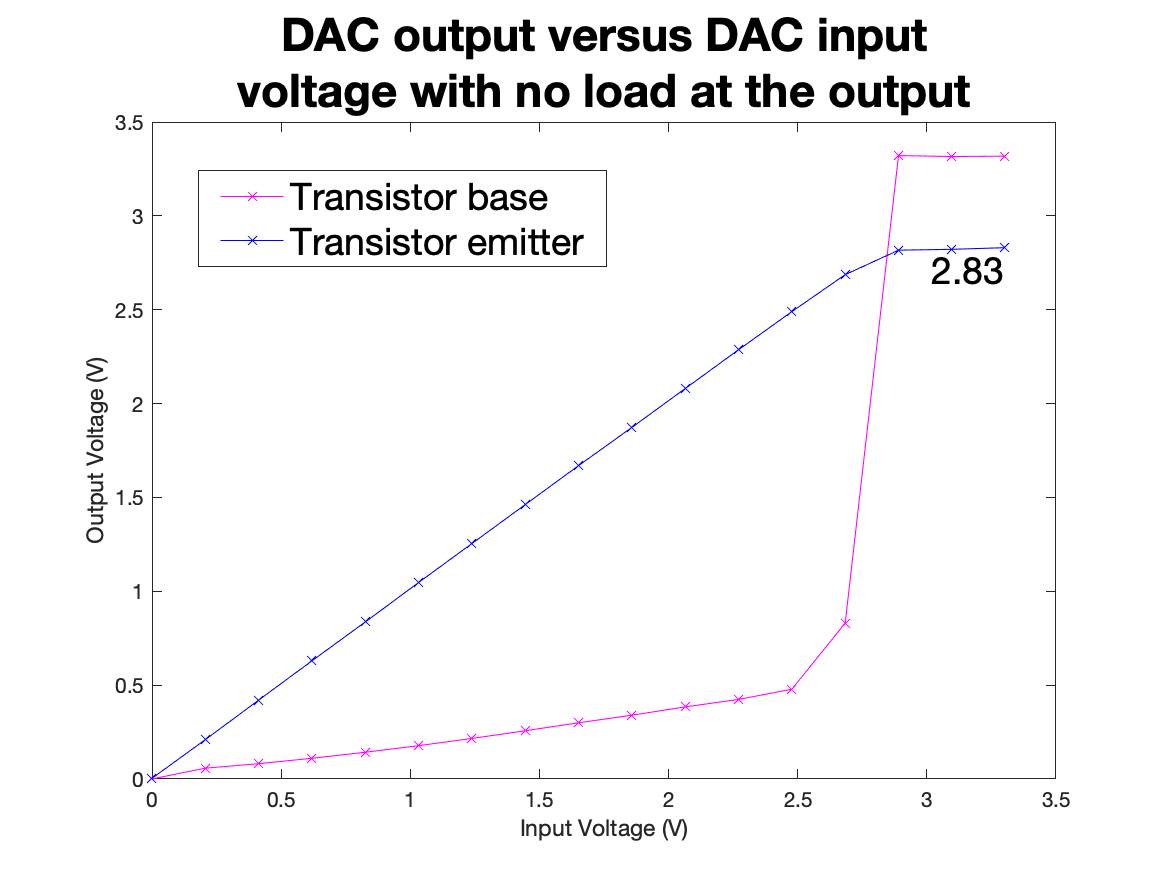
\includegraphics[width=\textwidth]{Figures/Testing/DAC_no_load}
        \caption{The input voltage versus the output voltage of the \gls{dac} with no load.}
        \label{fig:dac-voltage-range-no-load} %chktex 24
    \end{minipage}%
    \begin{minipage}{.5\textwidth}
        \centering
        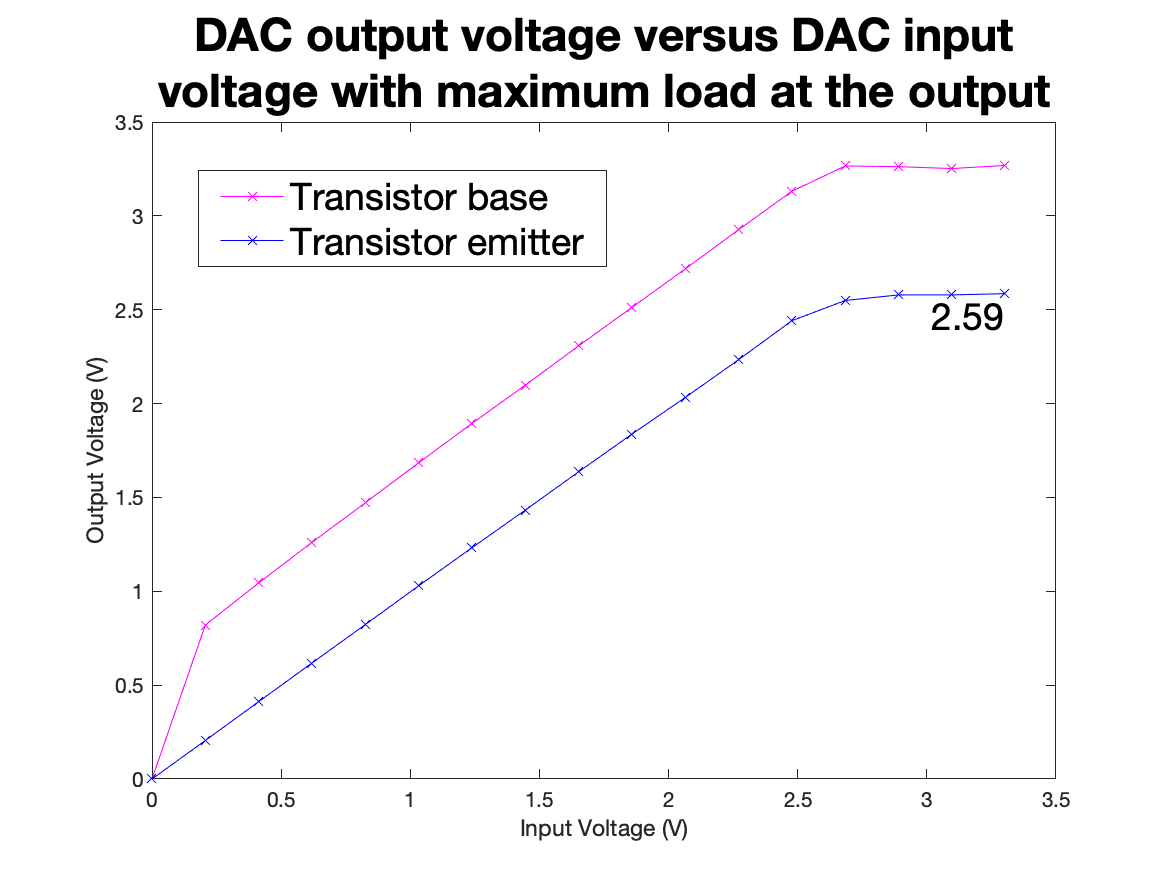
\includegraphics[width=\textwidth]{Figures/Testing/DAC_loaded}
        \caption{The input voltage versus the output voltage of the \gls{dac} with the maximum load of $100\Omega$.}
        \label{fig:dac-voltage-range-loaded} %chktex 24
    \end{minipage}
\end{figure}

The voltage drop due to $V_{BE}$ can clearly be seen on~\reffig{fig:dac-voltage-range-loaded}.
The unloaded output voltage reached $2,83V$, and the loaded output voltage reached $2,59V$, which were slightly higher than the predicted limits.

An alternative attempt was made to achieve a higher voltage output using the \gls{dac}'s internal voltage reference of $1,21V$ multiplied by a gain of $4$, resulting in a reference of $4,84V$.
As expected, this did not increase the output voltage; the base of the transistor continued to measure $3,3V$ and the emitter $2,83V$ while unloaded.

Due to the voltage limitations, the \gls{dac} was limited to $2,6V$ for future testing and implementation.
When excluding the voltage readings above $2,6V$, the \gls{dac} achieved a gain of $0,9837V/V$ and an offset $+0,0070V$ between the input voltage and measured voltage under maximum load. 
\section{ADC Accuracy}\label{sec:adc-accuracy}

The \gls{adc} was tested by measuring a range of voltages produced by the \gls{dac} and comparing them to the multimeter's measurement.
The \gls{adc} was configured in 12-bit mode, with each measurement taking 15 \gls{adc} clock cycles, equivalent to $250ns$ with the $16MHz$ system clock.
$5$ measurements were taken and averaged for each voltage outputted by the \gls{dac} to increase the accuracy of each measurement.
The results were graphed and shown in~\reffig{fig:adc-accuracy}. 

\begin{figure}[ht]
    \centering
    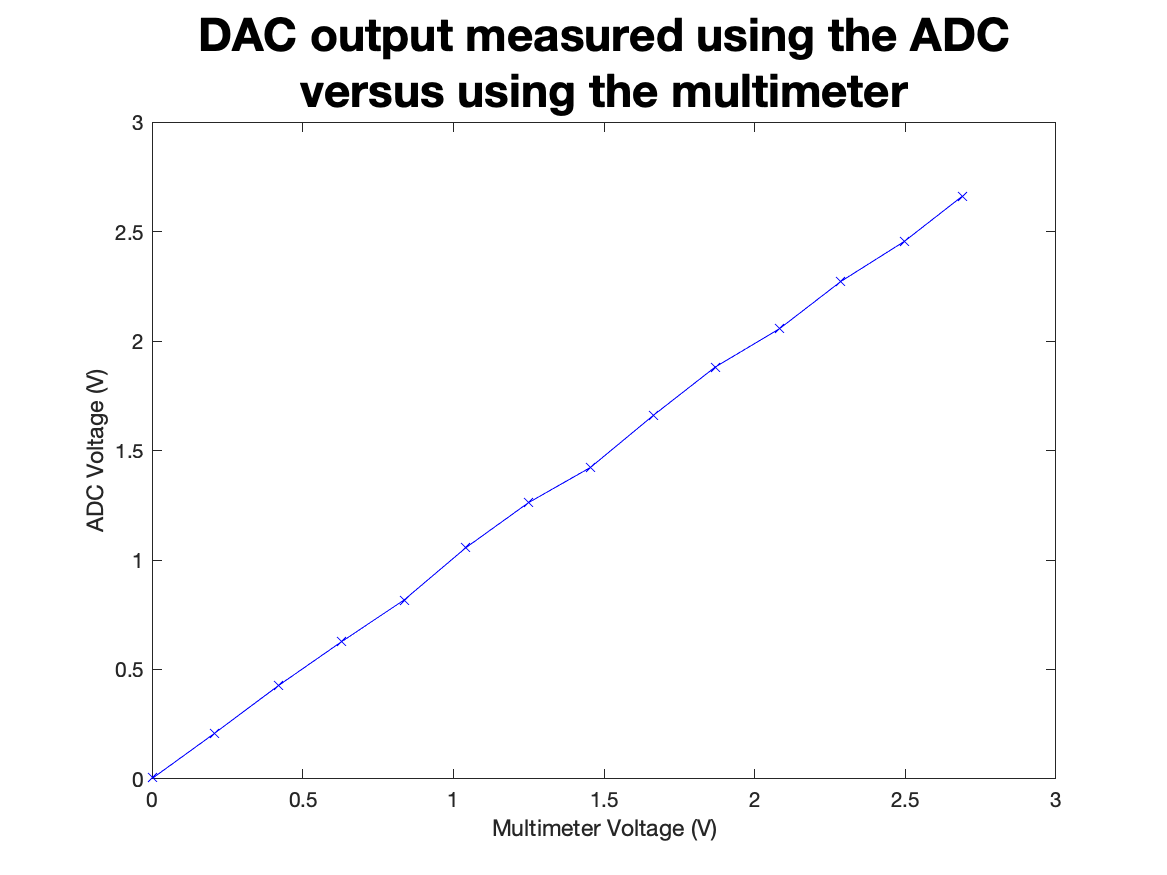
\includegraphics[width=0.5\textwidth]{Figures/Testing/ADC}
    \caption{The voltage output by the \gls{dac} measured by a multimeter versus by the \gls{adc}.}
    \label{fig:adc-accuracy} %chktex 24
\end{figure}

The \gls{adc} achieved a gain of $0,9877V/V$ and an offset of $0,0082V$ compared to the multimeter.

\section{Calibration Resistance}\label{sec:calibration-resistance}

The multimeter measured the calibration resistor by directly connecting its probes to the four parallel resistors.
The calibration resistor was electrically disconnected from the rest of the circuit during the measurement.
The calibration resistance was specified to be $5\Omega \pm 0,25\%$; thus, its actual value could range between $4,9875$ and $5,0125\Omega$.

The multimeter measured the calibration resistor to be $5,25\Omega$.
However, the multimeter probes measured $0,25\Omega$ when short-circuited.
Thus, the actual resistance was calculated as $5,00\Omega$.
It should be noted that the multimeter can only display to the nearest $0,01\Omega$.
Thus, the actual resistance could range from $4,995\Omega$ to $5,005\Omega$, and more precise equipment would be required to obtain a more accurate measurement.

\section{Resistance Measuring Accuracy}\label{sec:resistance-measuring-accuracy}

The probe's accuracy in measuring resistance was determined by comparing its calculated resistance to the multimeter's measurement of a given resistor.
The probe calculated resistance by measuring the voltage drop across the resistor attached between the titanium electrode ports and the calibration resistor. 
Then, it calculated its resistance per \refeqn{eqn:parallel-resistor-total} to \refeqn{eqn:parallel-resistor-uncertainty}.

For this test, the probe measured resistance using two methods: one with a single voltage provided by the \gls{dac} of $V_{DD}/2 = 1,65V$ and one with voltage sweep from the \gls{dac} with $50$ samples.
In the latter case, the resistances were calculated for each sample and averaged.
At low voltages, single-bit errors caused significant changes in the calculated resistance, which were avoided by limiting the voltage sweep to between $0,3V$ and $2,6V$.
The resistors used had a range of $0\Omega$, or a short-circuit, to $10\Omega$ as this is the expected range for the gold electrodes.
The results of the voltage sweep versus the multimeter test are shown in~\reffig{fig:resistance-measuring-accuracy-uncorrected}. 

\begin{figure}[!ht]
    \centering
    \begin{minipage}{.5\textwidth}
        \centering
        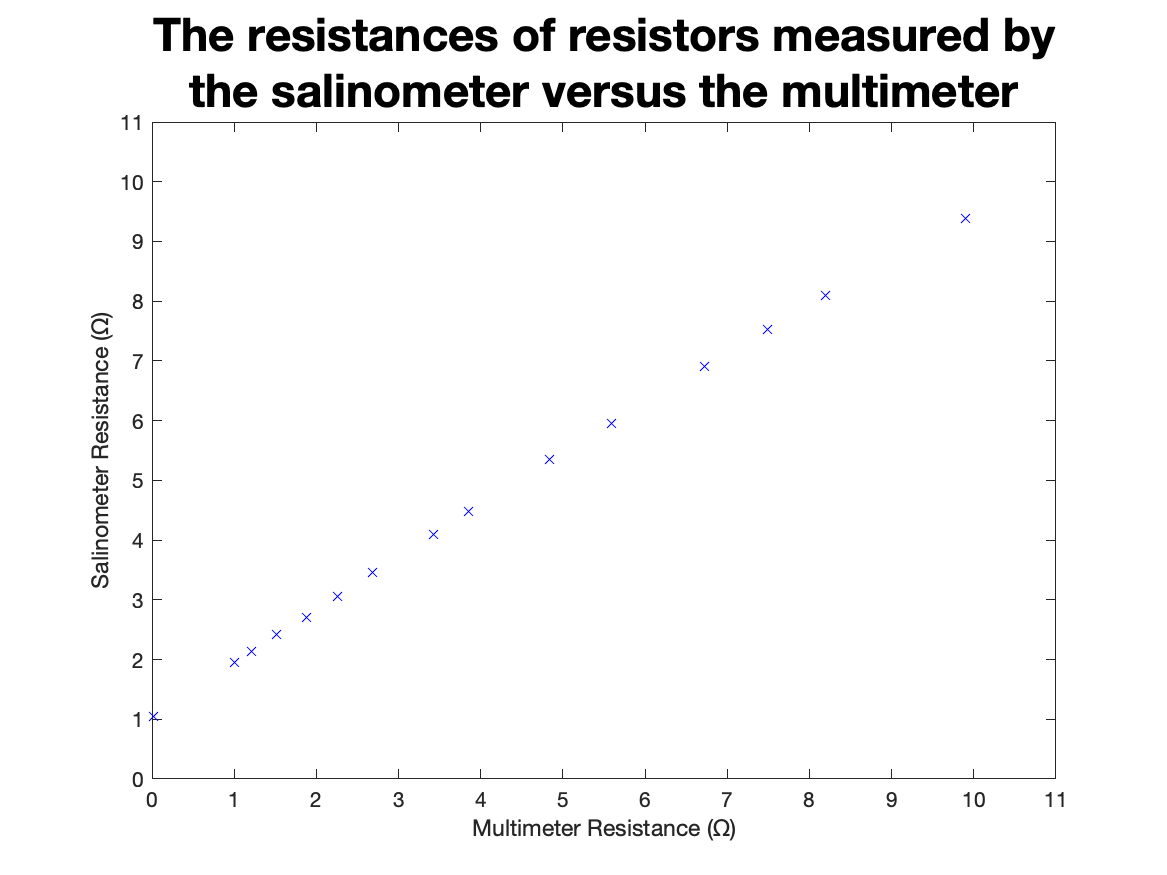
\includegraphics[width=\textwidth]{Figures/Testing/R_uncorrected}
        \caption{The resistance measuring test.}
        \label{fig:resistance-measuring-accuracy-uncorrected} %chktex 24
    \end{minipage}%
    \begin{minipage}{.5\textwidth}
        \centering
        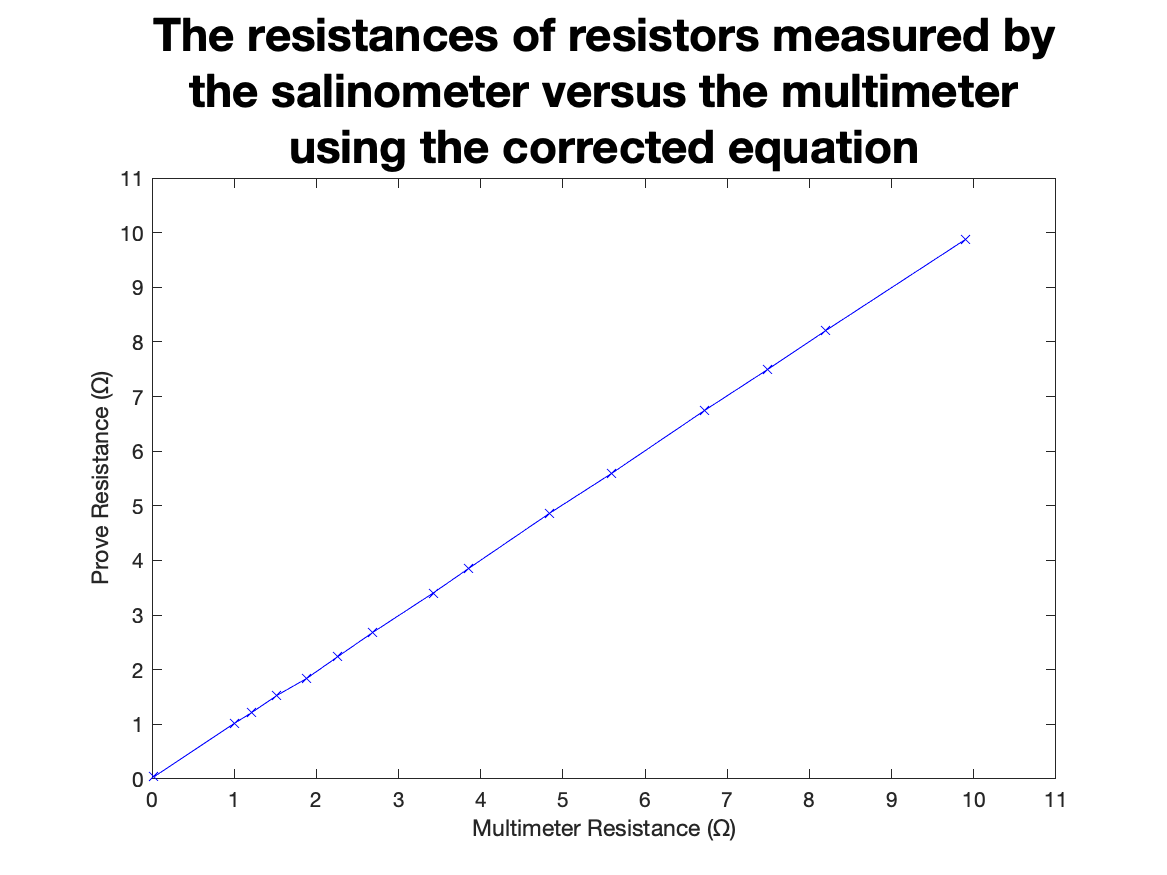
\includegraphics[width=\textwidth]{Figures/Testing/R_corrected}
        \caption{The resistance measuring test using the corrected equation.}
        \label{fig:resistance-measuring-accuracy-corrected} %chktex 24
    \end{minipage}
\end{figure}

The single voltage and voltage sweep methods were perfectly correlated with an $r^2$ value of $1,0000$.
However, there was a clear error between the probe's and the multimeter's measurements.
This error was assumed to be due to the unaccounted resistance of the switches and the traces.
While these values could be measured and included in the equation, a more efficient and arguably more accurate method would be to generate an equation of best fit and use it to calculate the correct resistance.

To determine the general formula of the equation of best fit, \refeqn{eqn:electrode-calib-resistance} with the electrode resistance $R_E$ and the calibration resistance $R_C$, was adjusted to include $r_e$, which represents the unknown resistance of the switches and traces as shown in \refeqn{eqn:resistance-measuring}.
$R_C$, $R_1$ and $r_e$ were condensed into the standard rational function coefficients $p$ and $q$ as shown in \refeqn{eqn:resistance-rational}.
Finally, the equation was rearranged to give the electrode's resistance in terms of the measured voltage ratio as shown in \refeqn{eqn:resistance-measuring-rational}.

\begin{align}
 V_{ratio} &= \lfrac{\lfrac{R_E + r_{e1}}{R_E + R_1 + r_{e2}}}{\lfrac{R_C + r_{e3}}{R_C + R_1 + r_{e4}}} \nonumber \\
    &= \lfrac{R_E + r_{e1}}{R_E + R_1 + r_{e2}} \times \lfrac{R_C + R_1 + r_{e4}}{R_C + r_{e3}} \label{eqn:resistance-measuring} \\
 V_{ratio} &= \lfrac{p_1 R_E + p_2}{R_E + q_1} \label{eqn:resistance-measuring-rational} \\
 R_E &= \lfrac{p_2 - q_1 V_{ratio}}{V_{ratio} - p_1} \label{eqn:resistance-measuring-rearranged}
\end{align}

The \refeqn{eqn:resistance-measuring-rational} of best fit was confirmed using MATLAB, which gave the values $p_1 = 17,4687$, $p_2 = 18,4643$ and $q_1 = 91,8315$ with an $r^2$ value of $1,0000$. 
The corrected resistance values were obtained from the previous data set by reversing the previous formula and applying \refeqn{eqn:resistance-measuring-rearranged} to the voltage ratios.
These results were graphed and are shown in \reffig{fig:resistance-measuring-accuracy-corrected} and have a gain of $1,0000$ and an offset of $0,0000$.
Note that this correction equation is only valid when $R_1$ is $100\Omega$ and separate equations will need to be generated should different values of $R_1$ be needed.

\section{Voltage Sweep Repeatability}\label{sec:voltage-sweep-repeatability}

The following tests investigate a method for producing repeatable voltage measurements of a saltwater sample.
In order to conduct these tests, the probe was cast into epoxy as described in \refsec{sec:probe-epoxy-casting}.

The tests were configured with parameters such as which electrodes to use, the voltage sample count, the \gls{adc} sample count and the \gls{dac} range.
Due to a circuit error discovered after the epoxy casting, the gold electrodes could only be used with the fringe guard.
Thus, the effectiveness of the fringe guard was unable to be tested.
Each voltage sweep results were transmitted over \gls{uart} to a computer, where they were processed using Microsoft Excel and MATLAB to generate graphs and metrics.

The first test was a voltage sweep performed both forwards and in reverse with increasing and decreasing \gls{dac} voltages respectively.
The test was configured with the gold electrodes and the fringe guard, 50 voltage samples, 2 \gls{adc} samples and a voltage range of $0-2,6V$.
It was performed on a salt water sample of unknown salinity around 30 \gls{psu}.
Ideally, the two sweeps should have been identical.
However, they were not, as shown in \reffig{fig:test1}.

\begin{figure}[ht]
    \begin{minipage}{0.5\textwidth}
        \centering
        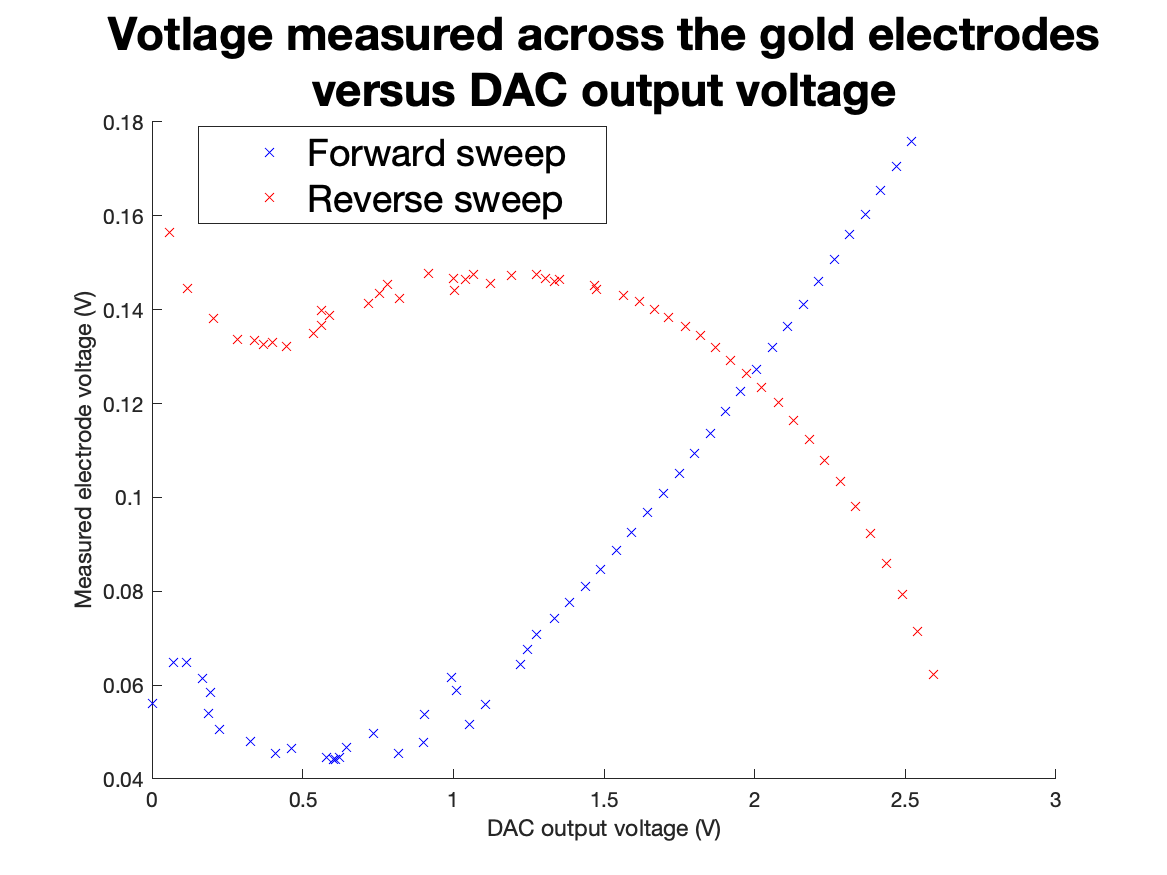
\includegraphics[width=\textwidth]{Figures/Testing/Aus2}
        \caption{Voltage sweep repeatability test 1 with gold electrodes and the fringe shield, a voltage range of $0-2,6V$, and 50 samples taken of salt water sample of unknown salinity.}
        \label{fig:test1} %chktex 24
    \end{minipage}
    \begin{minipage}{0.5\textwidth}
        \centering
        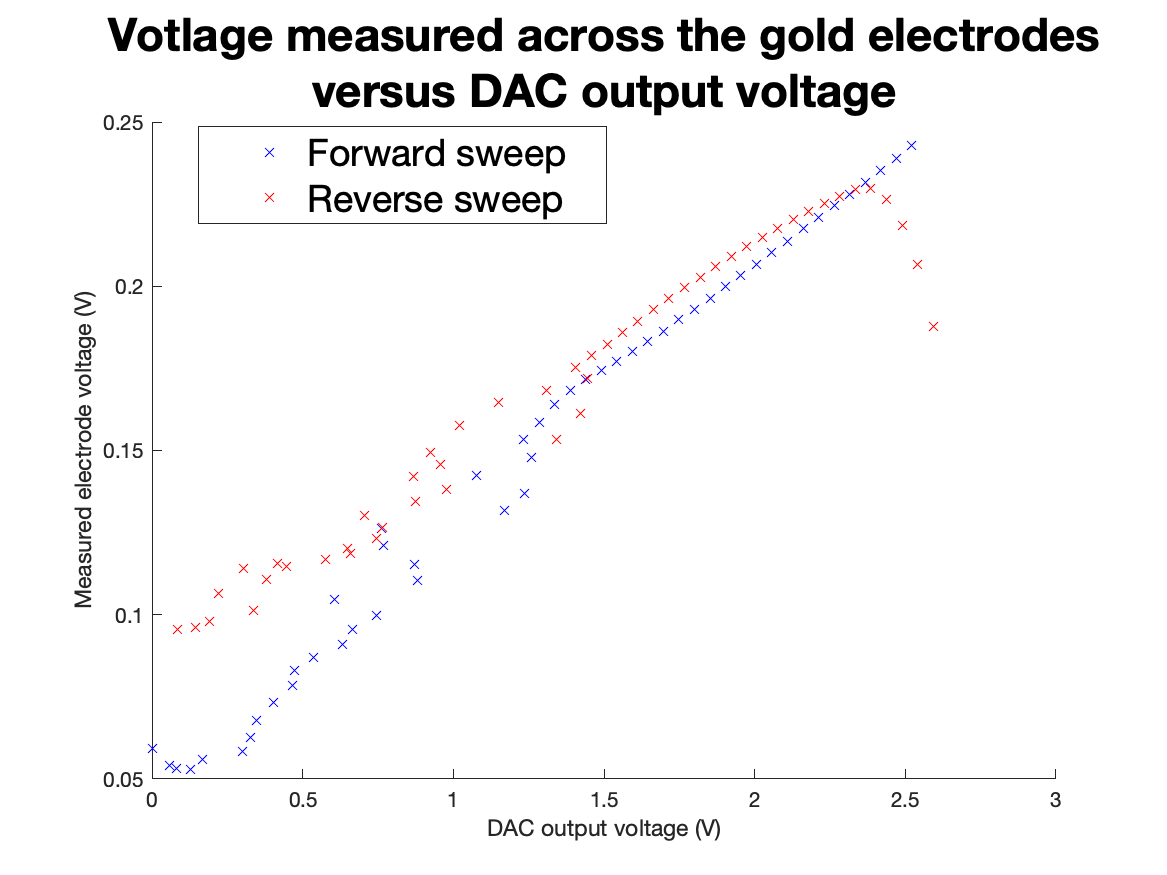
\includegraphics[width=\textwidth]{Figures/Testing/Aus3}
        \caption{Voltage sweep repeatability test 2 with draining and resetting the \gls{dac} between each voltage sample.}
        \label{fig:test2} %chktex 24
    \end{minipage}
\end{figure}

To further investigate the inconsistency, the \gls{dac} was reset to $0V$ before it was set to the desired voltage for each sample.
It should be noted that the \gls{dac} reset added a slight delay between each voltage sample of around $10ms$. 
While this did make the forward and reverse sweeps more similar, as shown in \reffig{fig:test2}, the initial voltage lag of the reverse sweep on the right hand-side of the graph was still present.

It was theorised that the measurements of the water briefly altered its properties, which in turn altered the proceeding measurements.
This alteration was unlikely to be a capacitive effect, as the measurements were taken bidirectionally, which would have dissipated any built-up charge.
It was possible that the voltage was dissociating the dissolved material into ions, allowing the charges in the salt water sample to move more freely and alter the measurement~\cite{ostdiek_inquiry_into_physics_2020}.
However, determining exactly what caused the alteration was beyond the scope of this project.

Instead, to further investigate this, a test was conducted taking priming measurements at the maximum voltage of $2,6V$ before capturing the actual measurements.
The priming caused the actual measurements in both directions to start high and progressively move to their predicted paths, as shown in \reffig{fig:test3}.

\begin{figure}[ht]
    \begin{minipage}{0.5\textwidth}
        \centering
        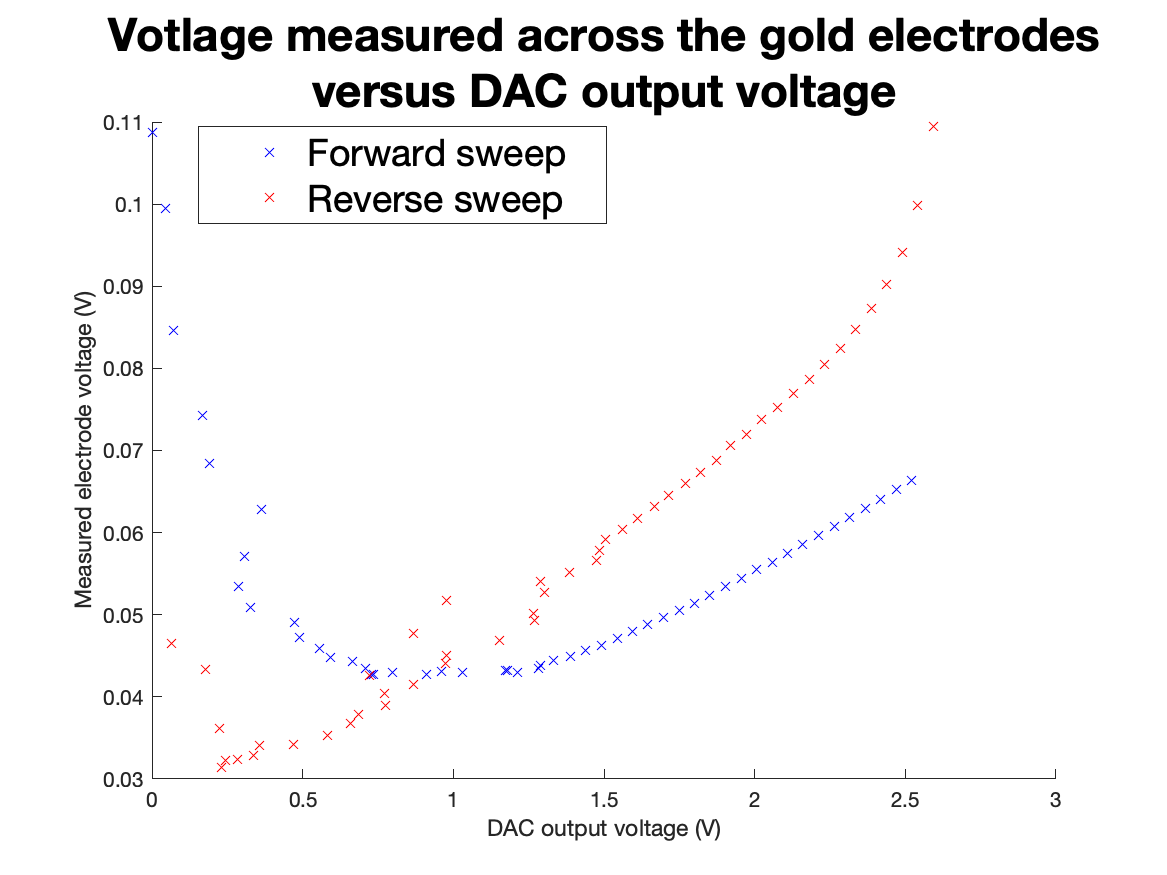
\includegraphics[width=\textwidth]{Figures/Testing/Aus5}
        \caption{Voltage sweep repeatability test 3 with 25 priming measurements taken before the actual measurement.}
        \label{fig:test3} %chktex 24
    \end{minipage}
    \begin{minipage}{0.5\textwidth}
        \centering
        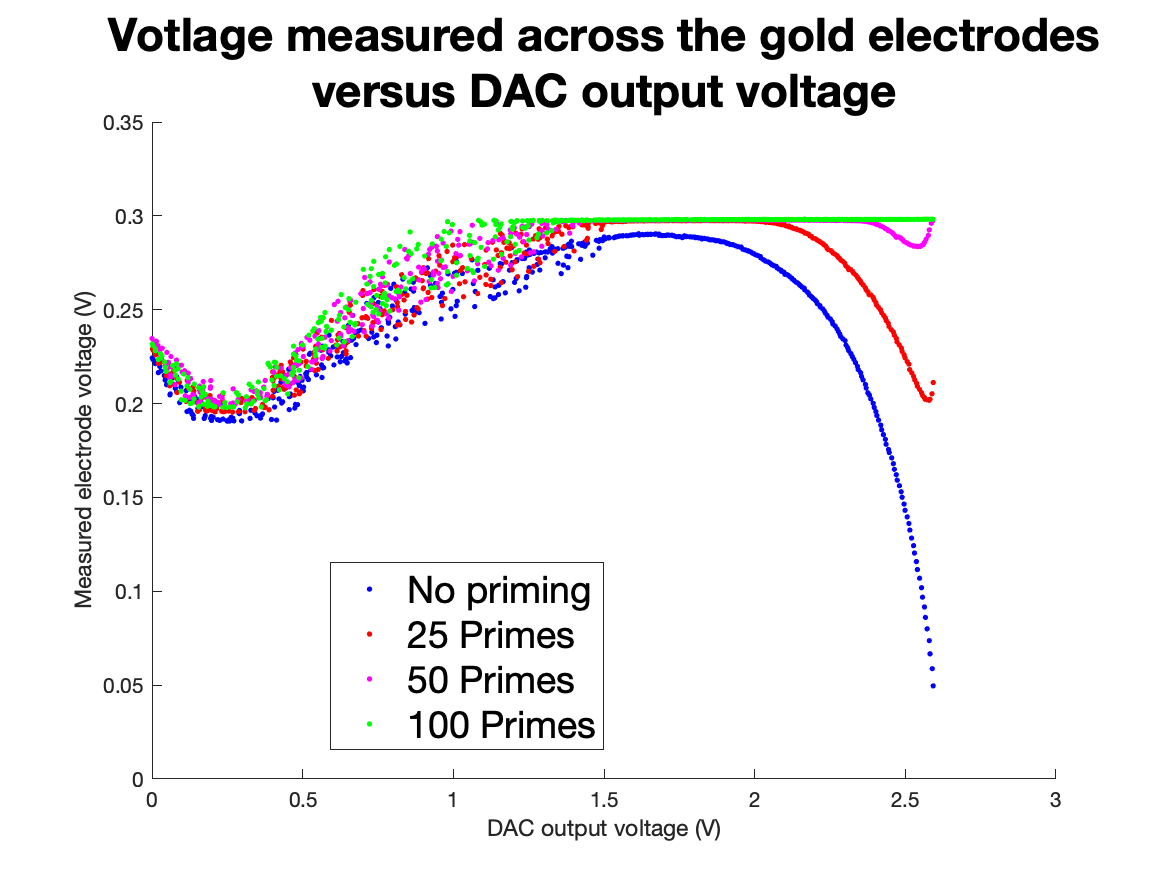
\includegraphics[width=\textwidth]{Figures/Testing/Aus7}
        \caption{Voltage sweep repeatability test 4 with a varying number of priming measurements and all true measurement taken as reverse voltage sweeps with 500 voltage samples.}
        \label{fig:test4} %chktex 24
    \end{minipage}
\end{figure}

This result supported the theory that the measurements were affecting the water.
The next test varied the number of priming measurements and used 500 voltage samples to increase the curve's resolution, as shown in \reffig{fig:test4}.
It should be noted that the voltage measurement effectively clipped at $0,3V$ as the output of the $11\times$ gain op-amp reached $0,3\times 11 = 3,3V$, which is the maximum voltage it can output.

While it was theoretically possible to perfectly prime a measurement, it was considered impractical, and it was also unlikely that the priming would have zero impact on the actual measurements.
Thus, voltage priming was not considered a viable solution for making repeatable measurements.
These results also indicated that a voltage measurement could be vulnerable to the priming effect from the previous measurement, which would cause undesirable effects.
Thus, an alternative method was needed to take the measurements.

It was noticed that the priming effect decreased over time, allowing the voltage sweeps in \reffig{fig:test3} to return to their expected curves.
A new theory stemmed from this that the water could relax from a primed state over time.
To test this, a delay, or relaxation time, was added between voltage samples, during which no voltage was applied to the electrodes.
The first test used a relaxation time of $2s$ and $500ms$.
With a $2s$ relaxation time, the forward and reverse voltage sweeps were near identical, as shown in \reffig{fig:test5}
However, with a $500ms$ relaxation time, there was a clear difference and the same initial voltage lag shown in \reffig{fig:test2}.

\begin{figure}[ht]
    \begin{minipage}{0.5\textwidth}
        \centering
        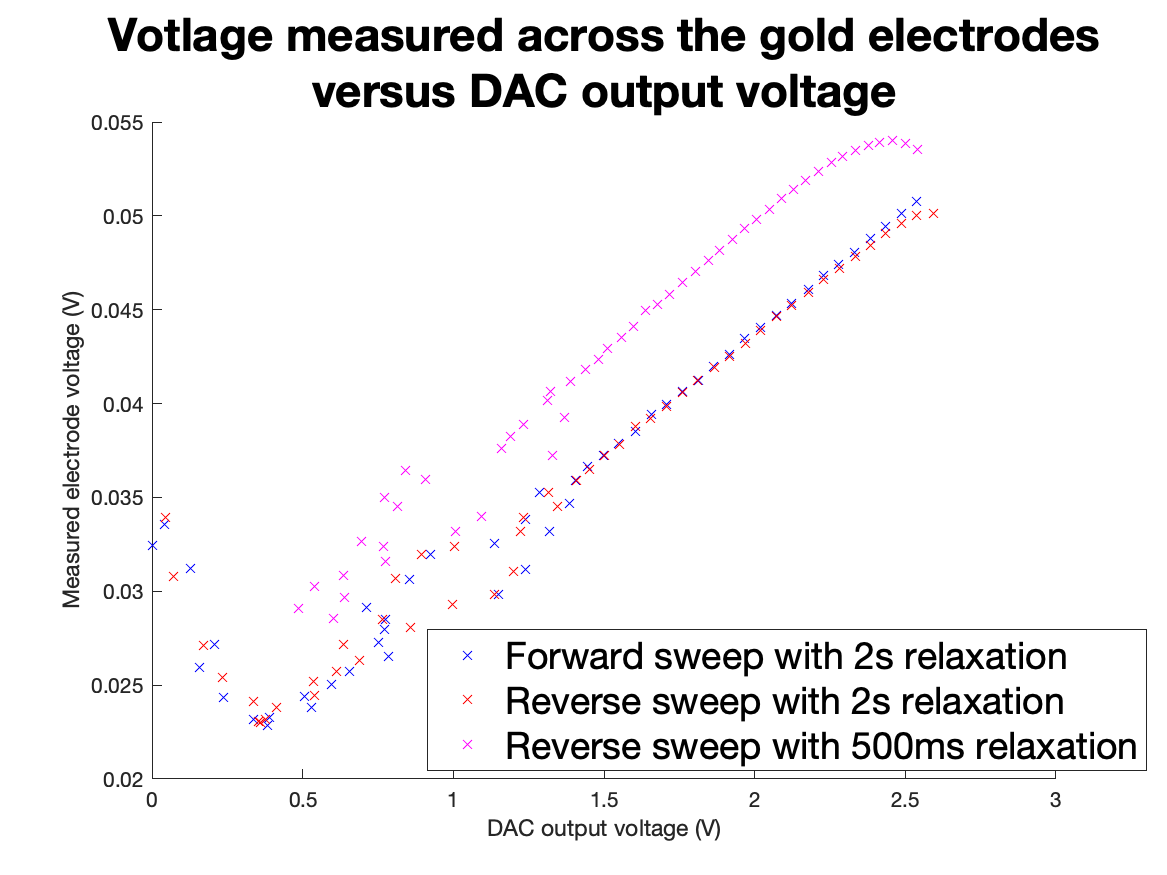
\includegraphics[width=\textwidth]{Figures/Testing/Aus8}
        \caption{Voltage sweep repeatability test 5 with a varying amount of relaxation time before each measurement was taken and 50 samples.}
        \label{fig:test5} %chktex 24
        \end{minipage}
    \begin{minipage}{0.5\textwidth}
        \centering
        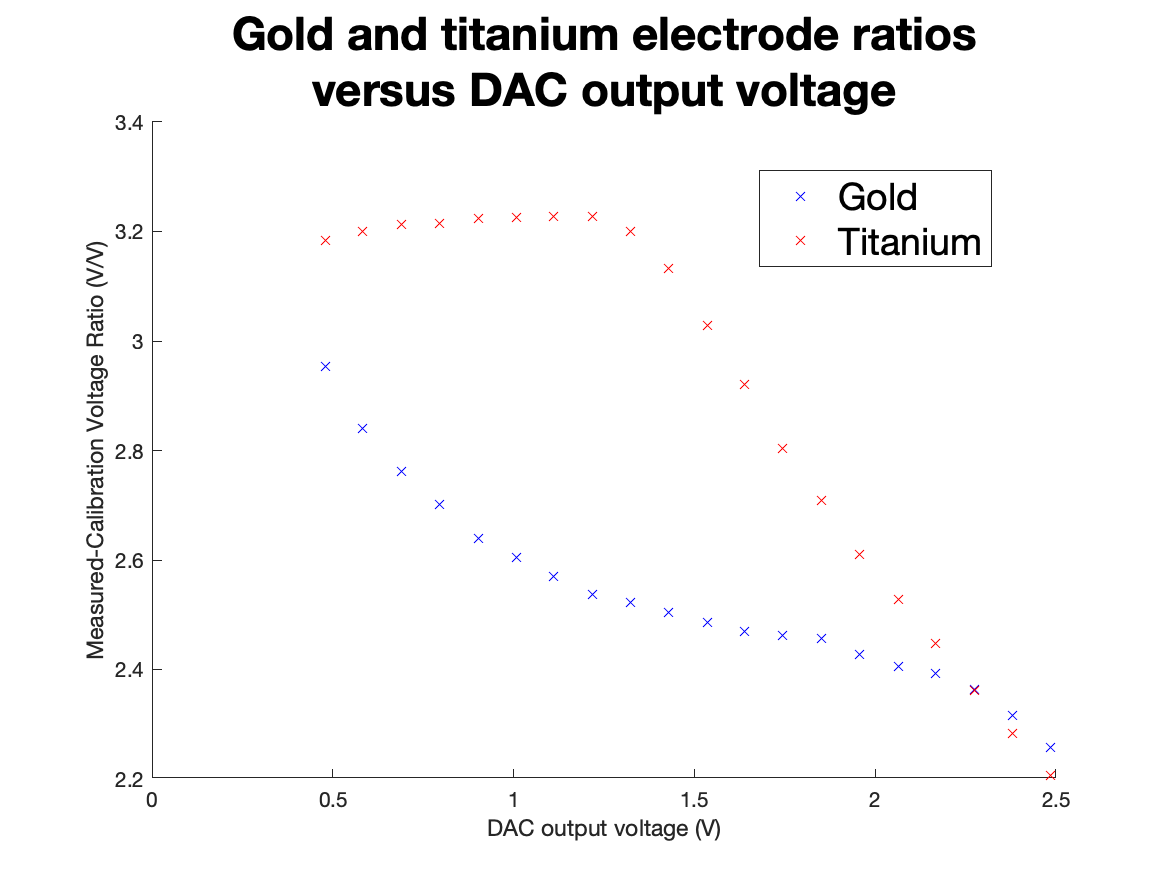
\includegraphics[width=\textwidth]{Figures/Testing/AusTi15}
        \caption{Voltage sweep repeatability test 6 with the difference between the titanium and gold electrodes.}
        \label{fig:test6} %chktex 24
    \end{minipage}
\end{figure}
This test concluded a valid method of measuring a voltage sweep, which used a relaxation time of $2s$ between each voltage sample.
This method allowed the titanium electrodes' length and spacing to be experimentally configured such that they could use the same $R_1$ value of $100\Omega$ as the gold electrodes.
Iterative testing revealed that a length of $30m$ and a spacing of $6mm$ used most of the $0V$ to $0,3V$ available to the electrodes.
A test comparing the titanium and gold electrodes was performed using a relaxation time of $2s$, shown in \reffig{fig:test6}.
The results showed that the gold electrodes followed the same curve that \refref{benjankar_ec_based_salt_measurement_2021} found, while the titanium electrodes did not.
The reason for this is unknown; it was theorised that the titanium electrodes' fringing effect and conductivity difference were the cause, but this needed further investigation.

The investigation into determining a repeatable voltage sweep necessitated two more tests: the repeatability of the sweep on the same sample and the differentiation between samples.
The former involved taking two voltage sweeps of two different saltwater samples of unknown but different salinities, shown in \reffig{fig:test7}.
These results showed that the voltage sweeps were approximately grouped by salinity, allowing for a clear differentiation between the two samples despite the noise in the measurements.

\begin{figure}[ht]
    \begin{minipage}{0.5\textwidth}
        \centering
        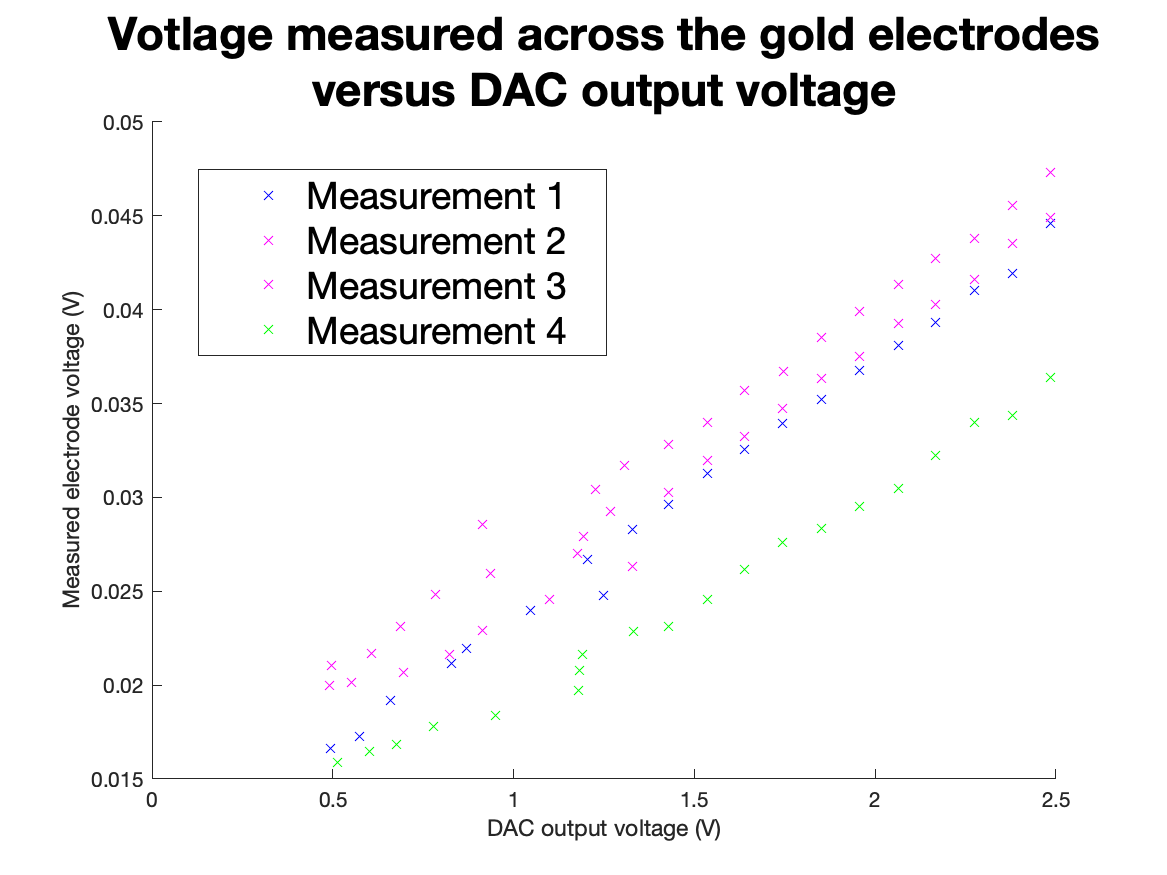
\includegraphics[width=\textwidth]{Figures/Testing/Aus12}
        \caption{Voltage sweep repeatability test 7 with 4 identical tests of 20 samples with 2s of relaxation time between measurements.}
        \label{fig:test7} %chktex 24
    \end{minipage}
    \begin{minipage}{0.5\textwidth}
        \centering
        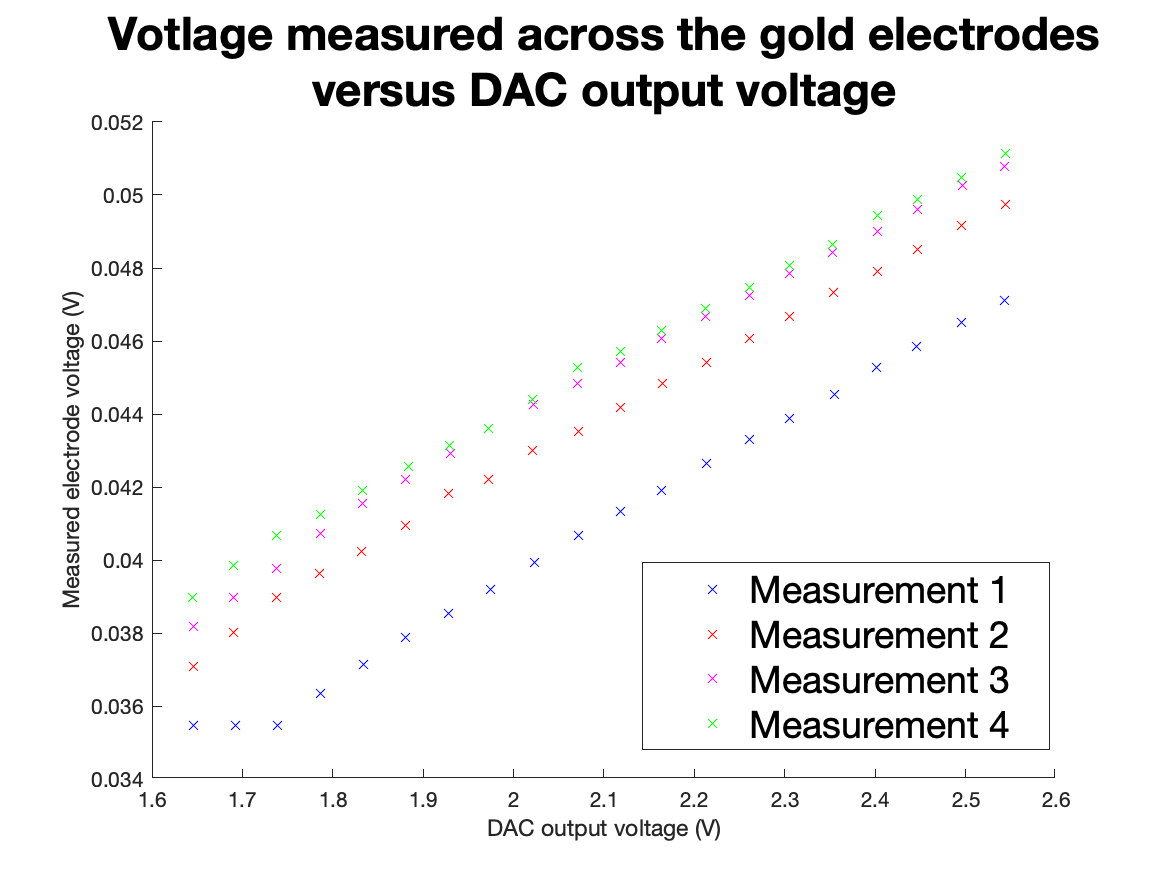
\includegraphics[width=\textwidth]{Figures/Testing/Aus10}
        \caption{Voltage sweep repeatability test 8 with 4 identical tests of 20 samples with 2s of relaxation time between measurements.}
        \label{fig:test8} %chktex 24
    \end{minipage}
\end{figure}

Next, an individual measurement's repeatability was further investigated by taking four identical voltage sweeps of the same saltwater sample.
The results, shown in \reffig{fig:test8}, showed that the measurements were approximately grouped.
However, it was noted that the voltage sweeps drifted upwards with each successive measurement.
A higher voltage sweep indicated a higher resistance, lower conductivity, and thus a lower salinity.
This was likely due to the previous sweep affecting the proceeding one, similar to the priming effect.
A test that could isolate both issues would be replacing the water between the electrodes during the voltage sweep.
This could be achieved using a pump and a large volume of water of known salinity, similar to how \href{https://oceanexplorer.noaa.gov/technology/ctd/ctd.html}{Ocean Exploration's CTD} operate. 
However, this apparatus was not available to this project.

It was noticed that there was a measurement inconsistency of the voltage samples below $1,5V$, which is visible in \reffig{fig:test5}.
However, the same inconsistency was present in the measurement and calibration reading. 
Thus, it was likely due to noise in the \gls{adc} or op-amp.
A similar inconsistency was present at the end of the voltage range, shown in \reffig{fig:test6}, likely due to the voltage lag of the reverse sweep.
Thus, to allow for a more straightforward analysis, the voltage sweeps of these voltages were excluded.

\section{Voltage to Conductivity Mapping}\label{sec:voltage-conductivity-mapping}

The following investigation aimed to determine the relationship between a saltwater sample's voltage sweep and conductivity.
This required samples of known salinity, which were created by mixing sea salt and distilled water.
A handheld salinometer, accuracte to $0,1$ \gls{psu}, was used to measure the samples, which were $24,4$, $29,1$, $32,9$ and $34,8$ \gls{psu}

In order to correctly assess the relationship between the voltage and conductivity, the probe had to calibrate on a standard solution of $35$ \gls{psu} at $15\degree C$ and $0dbar$.
$34,8$ was the closest value attainable to the required \gls{psu} using the equipment available.
This sample was placed in a fridge and cooled to below $15\degree C$, then removed and placed at room temperature where it warmed up. 
Once the sample reached approximately $15\degree C$, four voltage sweeps were taken with the gold and titanium electrodes using 20 voltage samples and 2s of relaxation, shown in \reffig{fig:test9} and \reffig{fig:test10}.

\begin{figure}[ht]
    \begin{minipage}{0.5\textwidth}
        \centering
        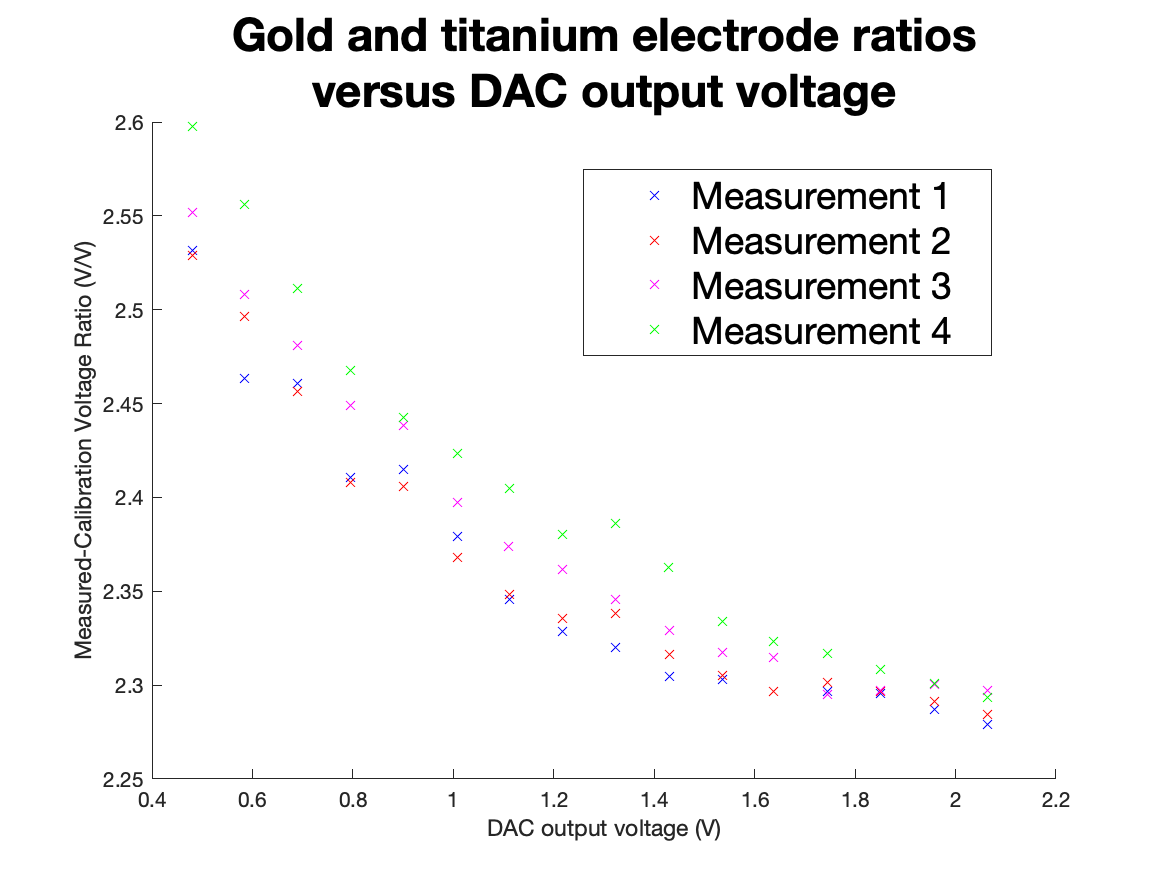
\includegraphics[width=\textwidth]{Figures/Testing/Aus16}
        \caption{Conductivity mapping test 1 with 4 tests using the gold electrodes and the fringe guard taken of a $34,8$ \gls{psu} sample at $15,0\degree C$.}
        \label{fig:test9} %chktex 24
    \end{minipage}
    \begin{minipage}{0.5\textwidth}
        \centering
        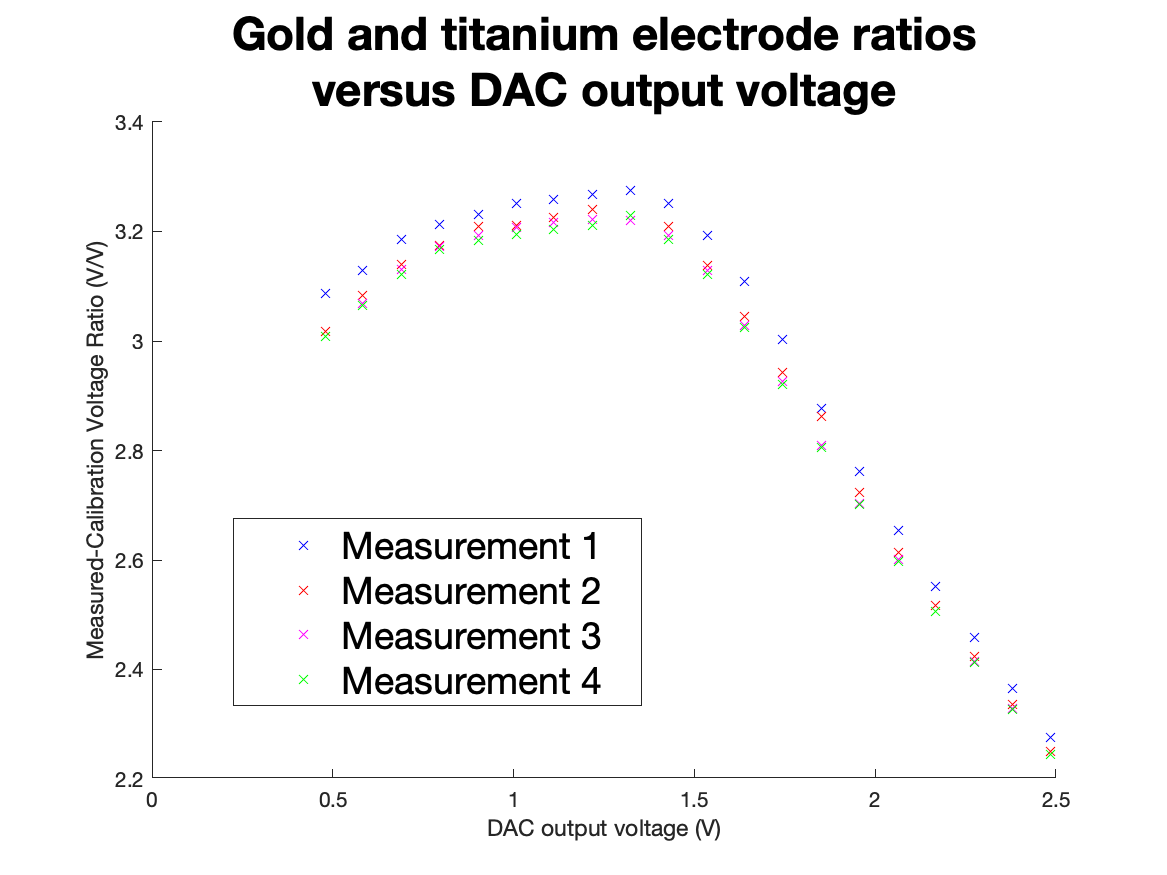
\includegraphics[width=\textwidth]{Figures/Testing/Ti16}
        \caption{Conductivity mapping test 2 with 4 tests using the titanium electrodes taken of a $34,8$ \gls{psu} sample at $15,0\degree C$.}
        \label{fig:test10} %chktex 24
    \end{minipage}
\end{figure}

The gold electrode test showed a similar result to \reffig{fig:test7}, where the measurements had the same shape and were approximately grouped, increasing with each successive test.
However, the titanium electrode test shows different results, appearing to have two different curves.
The samples taken below $1.4V$ appeared concave, while those above $1.4V$ appeared convex, which was confirmed not to be due to the voltage clipping at $0,3V$.
It was theorised that this was due to the fringing effect of the titanium electrodes, which were overlaid with the resistance-voltage curve of the saltwater sample.
However, this could not be verified, as the gold electrodes could not be tested without the fringe guards. 
Thus, the fringing effect could not be further studied.

Similar measurements were taken of the $24,4$ \gls{psu} and $29,1$ \gls{psu} samples, shown in \reffig{fig:test11} to \reffig{fig:test14}, to allow for a comparative analysis.
These tests were not conducted at $15\degree C$, which required their temperatures to be recorded and corrected for in the salinity equation.
All the tests were conducted at $0dbar$. 
Thus, pressure did not need to be corrected.

\begin{figure}[ht]
    \begin{minipage}{0.5\textwidth}
        \centering
        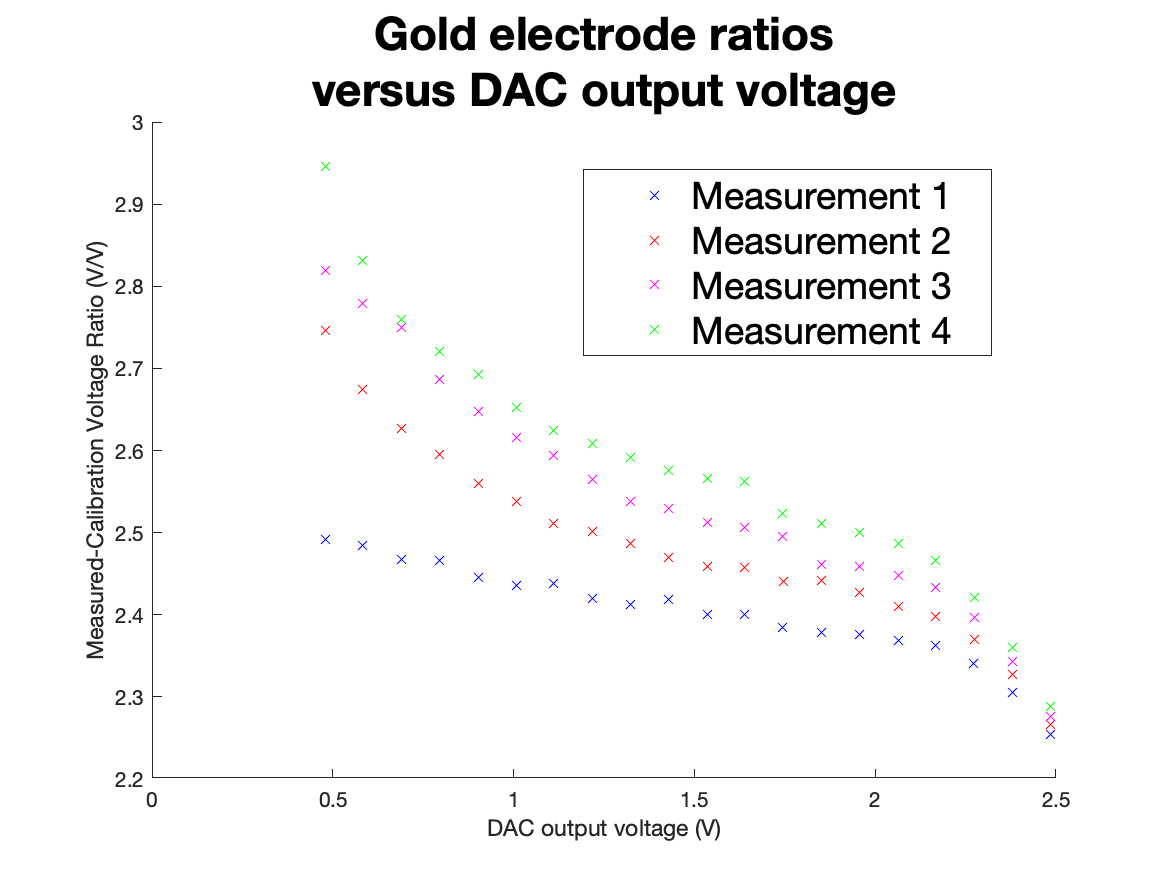
\includegraphics[width=\textwidth]{Figures/Testing/Aus17}
        \caption{Conductivity mapping test 3 with 4 tests using the gold electrodes and the fringe guard taken of a $24,4$ \gls{psu} sample at $21,7\degree C$.}
        \label{fig:test11} %chktex 24
    \end{minipage}
    \begin{minipage}{0.5\textwidth}
        \centering
        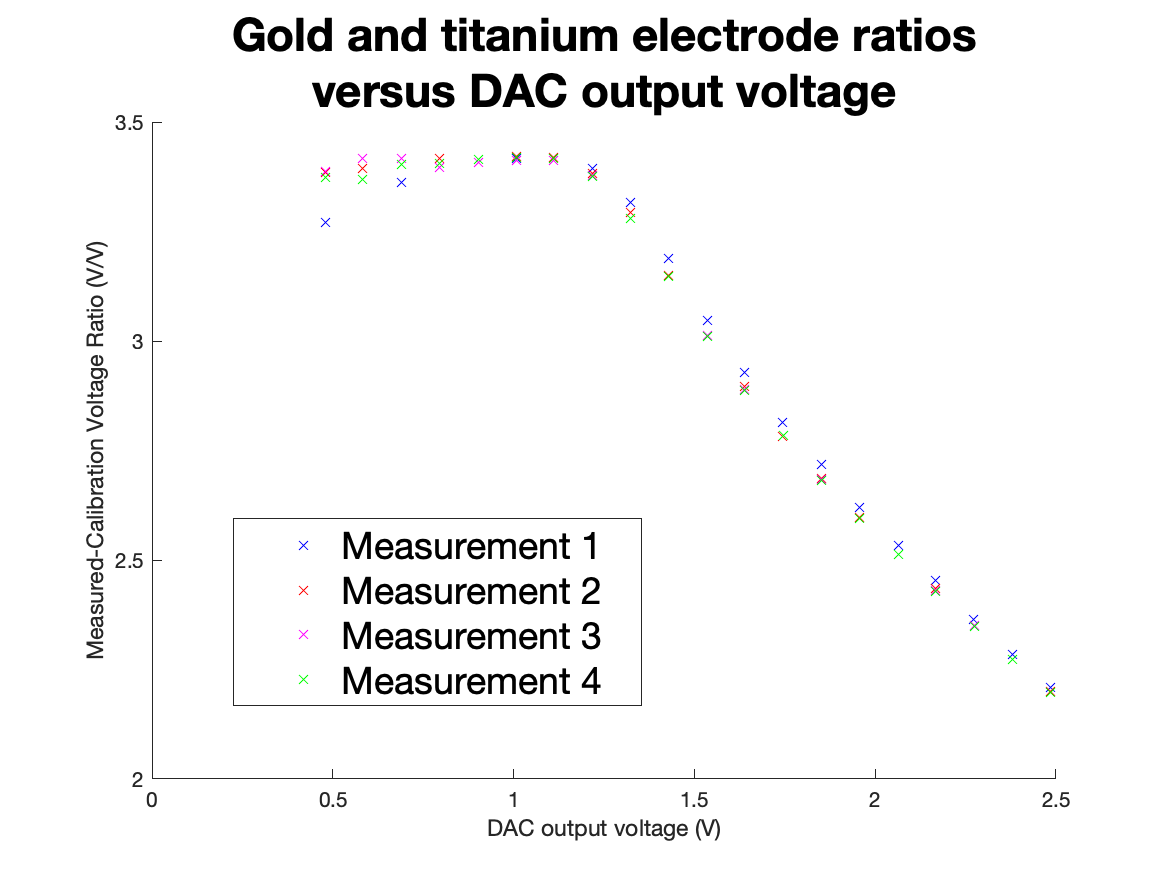
\includegraphics[width=\textwidth]{Figures/Testing/Ti17}
        \caption{Conductivity mapping test 4 with 4 tests using the titanium electrodes taken of a $24,4$ \gls{psu} sample at $21,7\degree C$.}
    \end{minipage}
\end{figure}

\begin{figure}[ht]
    \begin{minipage}{0.5\textwidth}
        \centering
        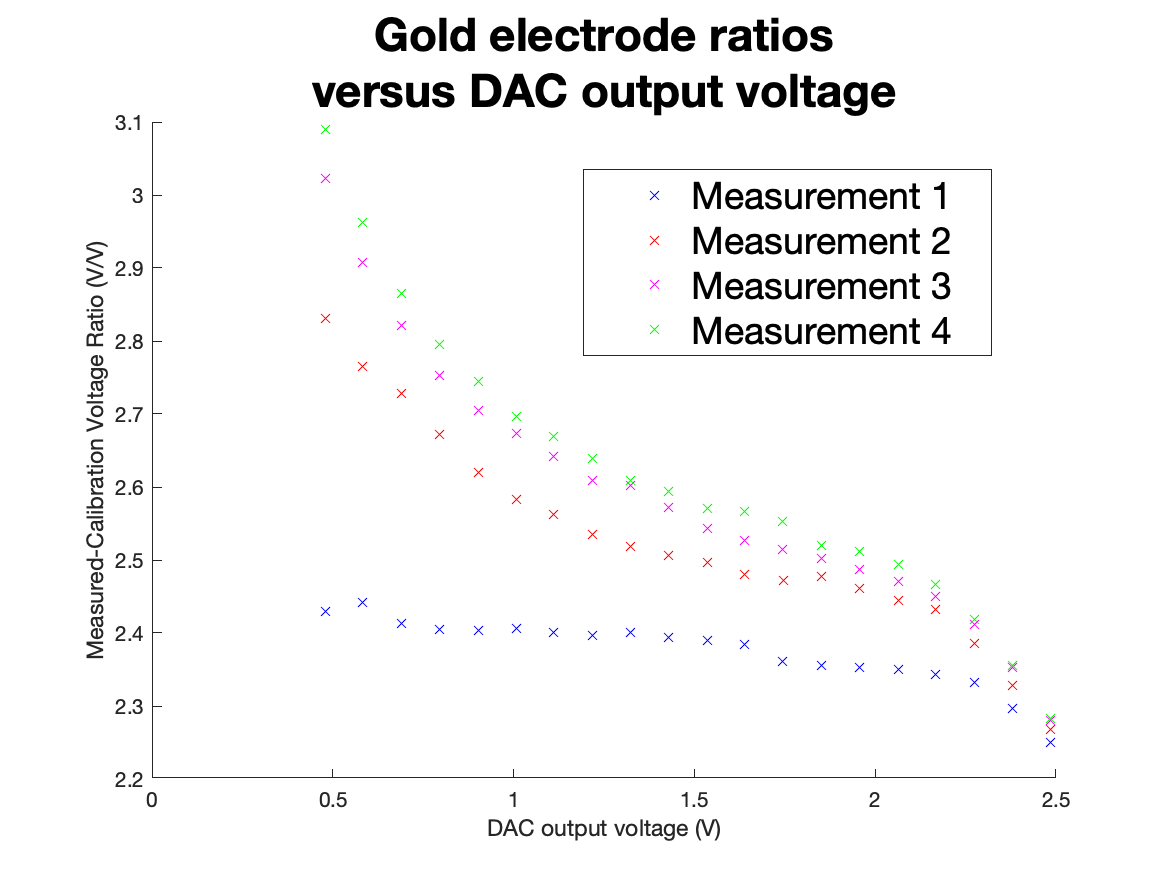
\includegraphics[width=\textwidth]{Figures/Testing/Aus18}
        \caption{Conductivity mapping test 5 with 4 tests using the gold electrodes and the fringe guard taken of a $29,1$ \gls{psu} sample at $20,2\degree C$.}
        \label{fig:test13} %chktex 24
    \end{minipage}
    \begin{minipage}{0.5\textwidth}
        \centering
        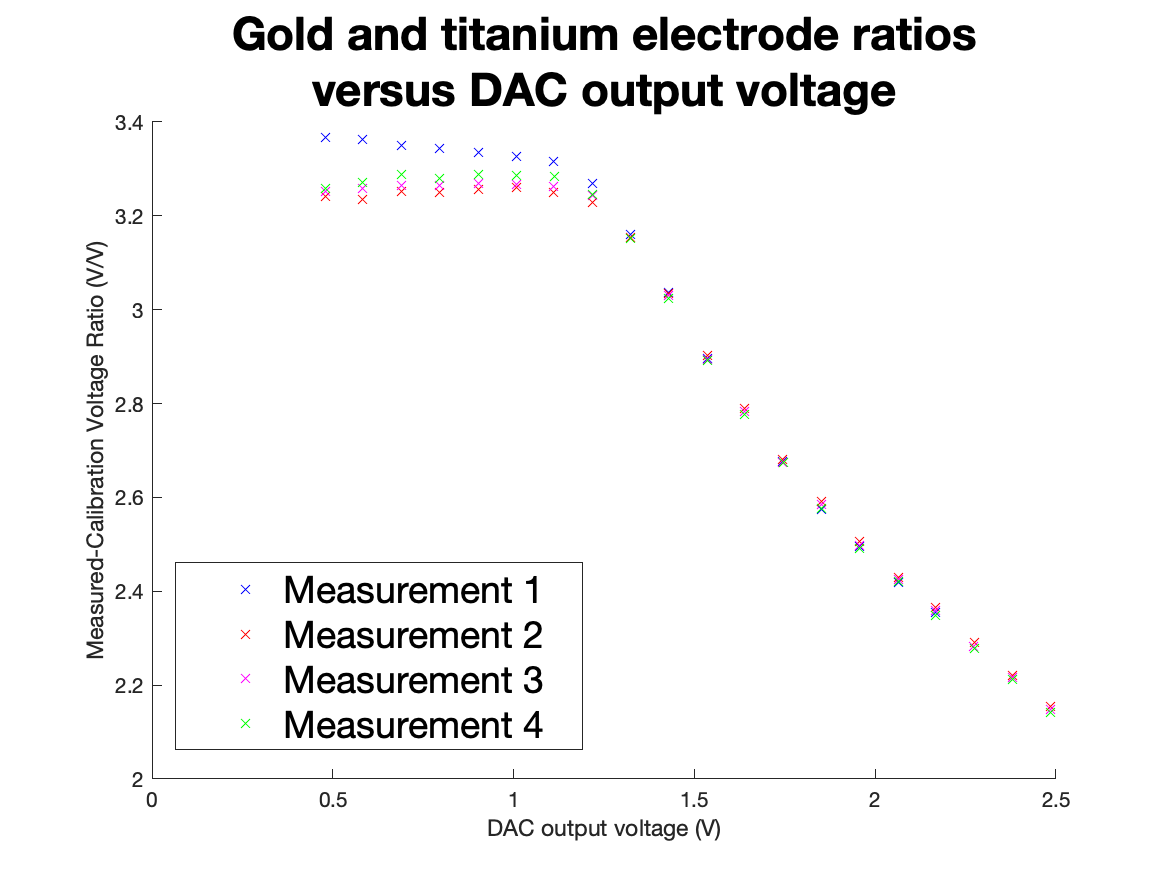
\includegraphics[width=\textwidth]{Figures/Testing/Ti18}
        \caption{Conductivity mapping test 6 with 4 tests using the titanium electrodes taken of a $29,1$ \gls{psu} sample at $20,2\degree C$.}
        \label{fig:test14} %chktex 24
    \end{minipage}
\end{figure}

These results showed a similar trend to the tests performed on the standard solution with the gold and titanium electrodes.
The gold electrodes continued to show variations between successive measurements, and it was noted that the titanium electrodes showed excellent consistency above $1,4V$.

To determine salinity, either a mathematical relationship between the curves and their salinity could be generated, or a metric from the equation of best fit could be taken as the effective conductivity.
The latter method was considered more straightforward and was attempted first.
The logical equation of best fit was a hyperbolic function, where the voltage ratio, measured voltage, and electrode resistance would approach infinity as the conductivity and salinity approach zero. 

The ideal hyperbole function $y = \frac{a}{x}$ was modified to include an offset $y = \frac{a}{x} + c$, as even with infinite conductivity, there would still be some resistance and voltage drop expected due to the switches and traces in the probe.
The equation parameters were calculated using MATLAB and graphed using the first measurement of each sample, shown in \reffig{fig:test15} and \reffig{fig:test16}.
The abnormalities at the higher voltages of gold electrode tests were removed, and the concave section of the titanium electrode tests below $1,4V$ was removed to allow for a more straightforward analysis.

\begin{figure}[ht]
    \begin{minipage}{0.5\textwidth}
        \centering
        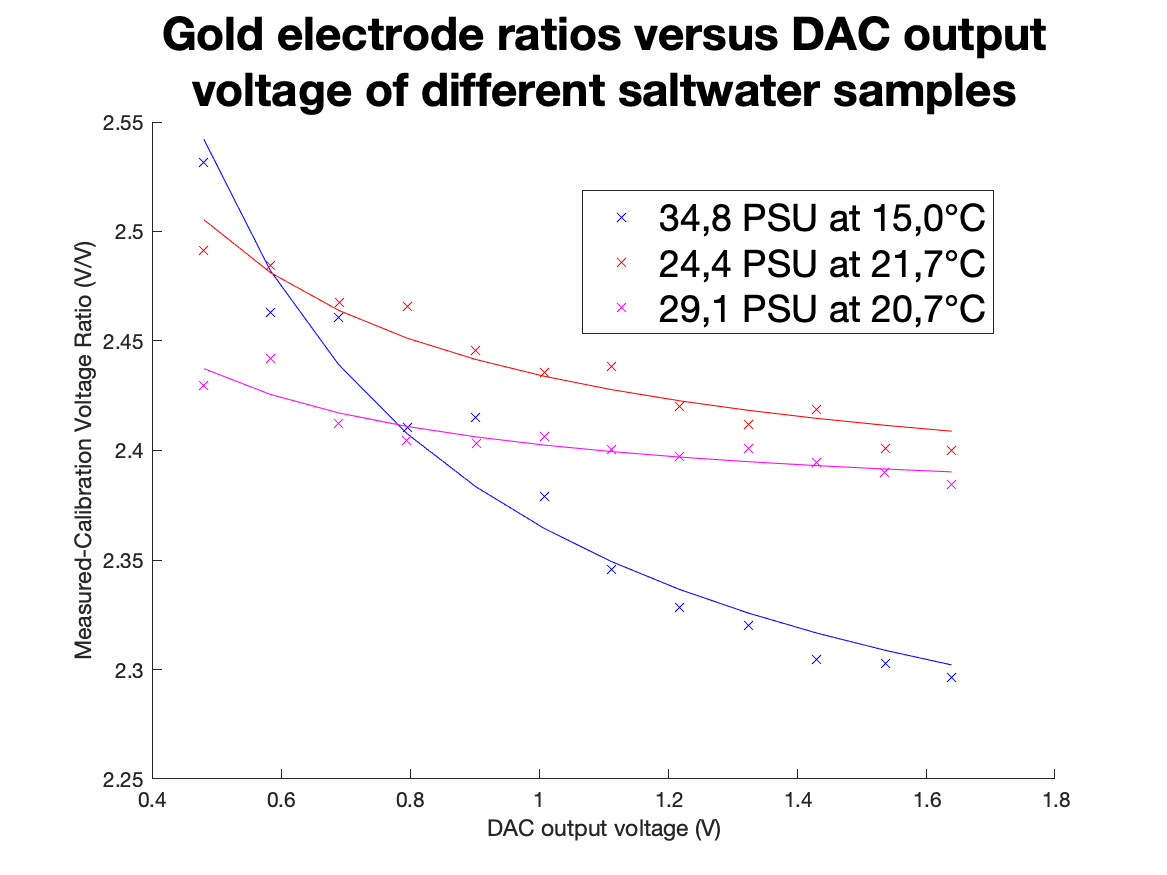
\includegraphics[width=\textwidth]{Figures/Testing/Au_sweep_analysis}
        \caption{The gold electrode tests of known samples with hyperbolic curves of best fit generated.}
        \label{fig:test15} %chktex 24
    \end{minipage}
    \begin{minipage}{0.5\textwidth}
        \centering
        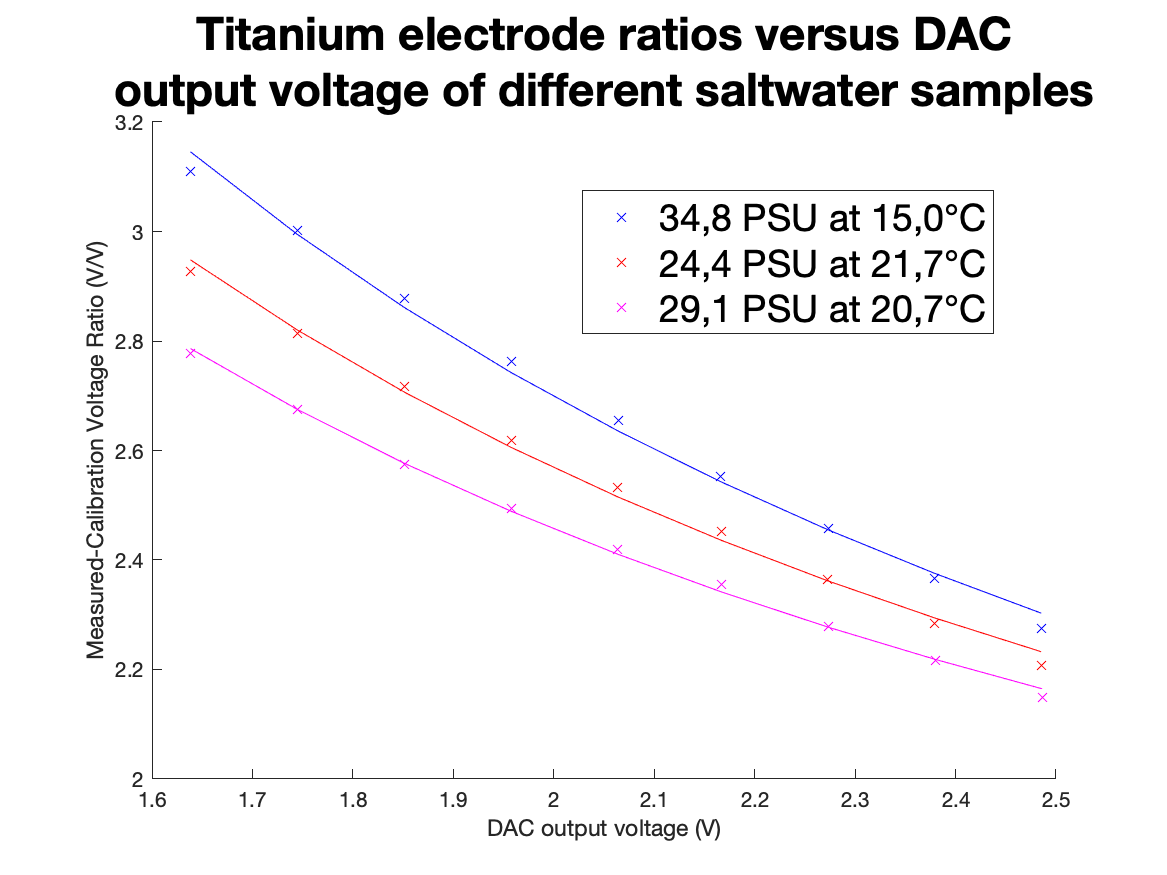
\includegraphics[width=\textwidth]{Figures/Testing/Ti_sweep_analysis}
        \caption{The titanium electrode tests of known samples with hyperbolic curves of best fit generated.}
        \label{fig:test16} %chktex 24
    \end{minipage}
\end{figure}

The gold and titanium electrode tests of the $24,4$ and $29,1$ \gls{psu} samples measured at similar temperatures showed a logical difference between their voltage sweeps, where the lower salinity sample had a higher voltage ratio.
However, the $34,8$ \gls{psu} did not follow this, likely due to its temperature change, which would have lowered its conductivity~\cite{stewart_introduction_to_physical_oceanography_2004}.

The gain value $a$ was calculated for each of these curves.
Higher salinities appeared to have lower $a$ values; thus, they were inverted before calculating salinity.
These values and their corresponding salinities are shown in \reftbl{tab:salinity-from-sweep}.
While these results return relatively higher values for higher salinity samples, they were required to be more accurate.
Attempts were made by raising the $a$ value to different powers, using the $c$ value, and linear offsets to $a$, but none resulted in correct salinity values.
It should be noted that multiplying the $a$ was ineffective, as salinity is calculated based on the ratio of two different $a$ values.

\begin{longtblr}[
    caption = {The gain values $a$ of the hyberbolic curve of best fits and the calculated salinities.},
    label = {tab:salinity-from-sweep},
]
{
    hlines,
    vlines, 
    colspec = {*{5}{X[c,m]}}
}
\textbf{Electrode} & \textbf{Sample Salinity (\gls{psu})} & \textbf{Gain Value $a$} & \textbf{Temperature ($\degree C$)} & \textbf{Calculated Salinity (\gls{psu})} \\
Gold & $34,8$ & $0,1631$ & $15,0$ & - \\
Gold & $24,4$ & $0,0656$ & $21,7$ & $84,9$ \\
Gold & $29,1$ & $0,0320$ & $20,2$ & $226,6$ \\
Titanium & $34,8$ & $4,0506$ & $15,0$ & - \\
Titanium & $24,4$ & $3,4400$ & $21,7$ & $35,7$ \\
Titanium & $29,1$ & $2,9851$ & $20,2$ & $43,4$ \\
\end{longtblr}

This investigation concluded that the probe could detect a clear and logical difference between salinity samples, but calculating salinity using the measurements proved inaccurate.
While further investigation could be conducted into determining a mathematical relationship between the curves and their respective conductivities, it was considered viable only with more accurate data attained through the previously mentioned method of pumping water over the electrode.
Thus, alternative methods were investigated.

\section{Individual Voltage Measurements}

A second approach, similar to that of \refref{instructables_water_salinity_meter}, was investigated, which used a single voltage measurement to calculate the salinity.
While this would prevent any impact of the priming effect, a single measurement is highly vulnerable to noise and errors, which could cause inaccuracies in the salinity calculation.
Tests were conducted with the gold electrodes and the fringe guard with the \gls{dac} set at $1,65V$, as this voltage appeared to be the most stable from the previous tests.
Similar to \refsec{sec:voltage-conductivity-mapping}, a standard solution of $34,8$ \gls{psu} was measured at $15\degree C$ and $0dbar$. 
Then, measurements of the other three samples were taken, and their temperatures were recorded.
The results are shown in \reftbl{tab:individual-voltage-measurements}.

\begin{longtblr}[
        caption = {The individual voltage measurements taken of different salt water samples.},
        label = {tab:individual-voltage-measurements},
    ]
    {
        hlines,
        vlines, 
        colspec = {*{5}{X[c,m]}}
    }
    \textbf{Sample Salinity (\gls{psu})} & \textbf{Voltage Ratio ($V/V$)} & \textbf{Calculated Resistance ($\Omega$)} & \textbf{Temperature ($\degree C$)} & \textbf{Calculated Salinity (\gls{psu})} \\
    $34,8$ & $2,178$ & $11,87$ & $15,0$ & - \\
    $24,4$ & $2,320$ & $12,79$ & $23,7$ & $24,9$ \\
    $29,1$ & $2,288$ & $12,62$ & $23,7$ & $25,5$ \\
    $32,9$ & $2,058$ & $11,06$ & $23,7$ & $32,2$ \\
\end{longtblr}

The voltage ratio was calculated for each sample, followed by its resistance using the correct resistance equation,\refeqn{eqn:resistance-measuring-rearranged}, determined in \refsec{sec:resistance-measuring-accuracy}.
The salinity was then calculated using the resistances.
Calculating conductivity using resistance was a scalar operation and thus was omitted as it does not affect the salinity calculation, as previously mentioned.
While these values proved more accurate in estimating salinity than the voltage sweep, they were inconsistent and subject to noise and error.

\section{AC Voltage Measurements}

A third approach, similar to that of \refref{jonsson_chip_based_salinity_2013}, was investigated, which used an \gls{ac} sine wave to measure the saltwater's response.
A sine wave was generated by writing precalculated values of a half sin wave to the \gls{dac} and changing the current direction between the electrodes every half wave, which gave the effect of a full sine wave centred around ground.
\Gls{adc} measurement were taken every time the \gls{dac} voltage was updated.
A slight, configurable delay was added between each \gls{dac} updated to allow the frequency of the sine wave to be controlled.
It should be noted that the probe was optimised for measuring \gls{dc} voltages, which required capacitors connected in parallel with the electrodes, which could not be removed after the probe was cast in epoxy.
These capacitors likely affected the saltwater's measured response.

A sine wave test was performed on the $32,9$ \gls{psu} sample using the titanium electrodes, shown in \reffig{fig:test17}.
Due to the circuit errors previously mentioned, the gold electrodes could not perform this test.
The sample had a phase delay in response to the sine wave.
However, when the sine wave crossed $0V$, the response would return to $0V$ as well. 
This was assumed to be due to the \gls{dac} draining the voltage from across the electrode when it crossed ground.
Additionally, the amplitude of the sample's response appeared to migrate indicating that it had not stabilised.

\begin{figure}[ht]
    \begin{minipage}{0.5\textwidth}
        \centering
        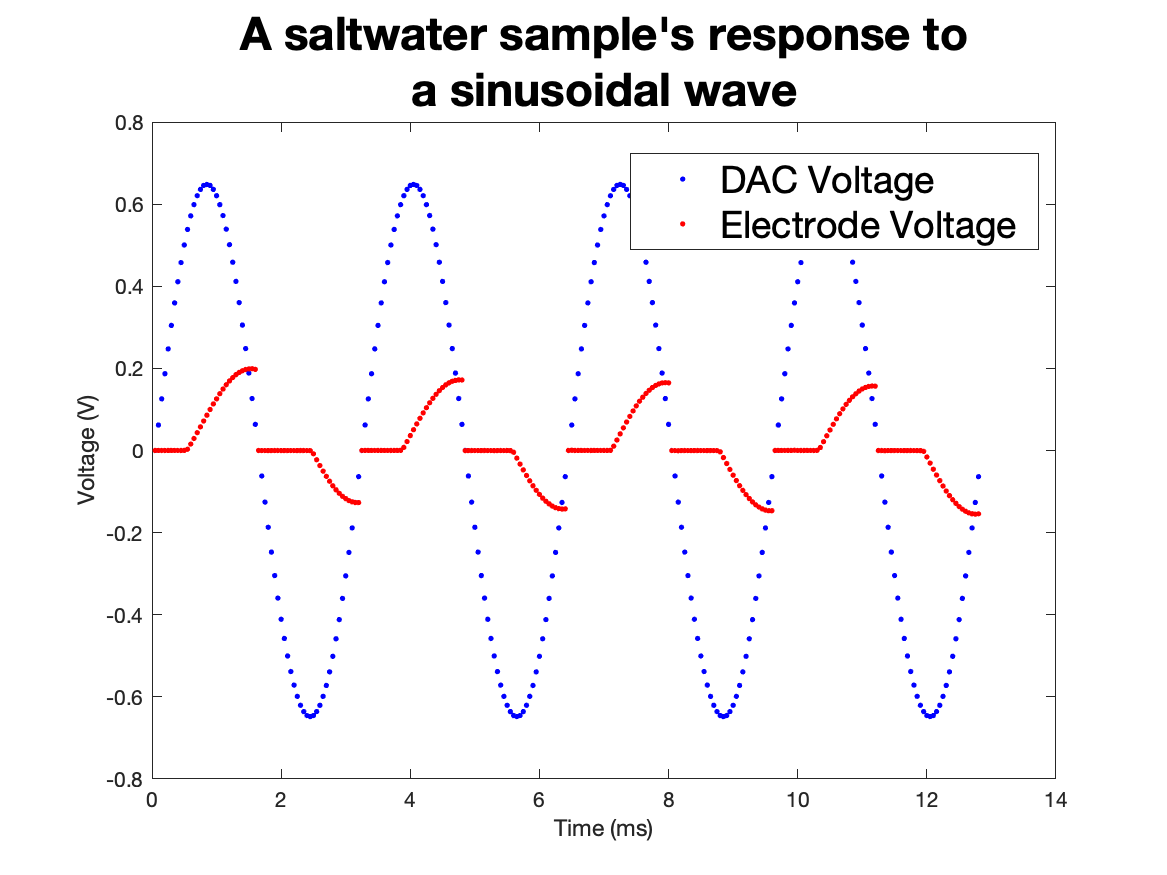
\includegraphics[width=\textwidth]{Figures/Testing/TiAC1}
        \caption{\gls{ac} test 1 with a 4 sine waves centred at $0V$.}
        \label{fig:test17} %chktex 24
    \end{minipage}
    \begin{minipage}{0.5\textwidth}
        \centering
        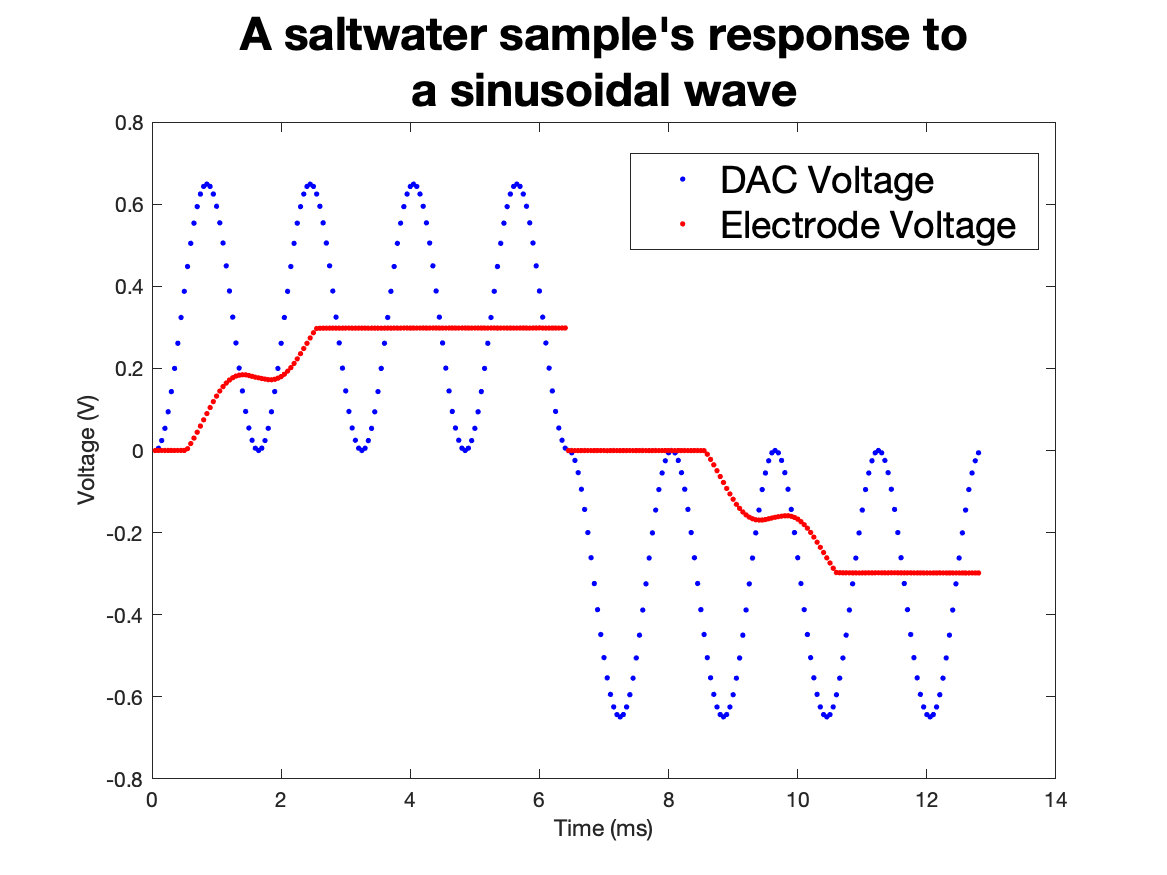
\includegraphics[width=\textwidth]{Figures/Testing/TiAC2}
        \caption{\gls{ac} test 1 with a 4 sine waves centred at $1,65V$ and 4 sine waves centred at $-1,65V$.}
        \label{fig:test18} %chktex 24
    \end{minipage}
\end{figure}

A second test was conducted with the sine wave centred at $V_{CC}/2 = 1,65V$, which prevented the \gls{dac} from draining the voltage from the electrodes.
The sine waves were repeated in both directions to prevent excessive corrosion of the electrode.
The results, shown in \reffig{fig:test18}, show the response of the sine wave saturates with a similar effect to the priming experienced with the voltage sweeps.
Thus, this test was considered not viable for salinity calculation.

Further tests centred at $0V$ were conducted on the $34,8$ and $24,4$ \gls{psu} samples.
To allow the drift of the peaks seen in \reffig{fig:test17} to settle, 75 sine wave measurements were performed before the actual measurement was taken, shown in \reffig{fig:test19} and \reffig{fig:test20}.

\begin{figure}[ht]
    \begin{minipage}{0.5\textwidth}
        \centering
        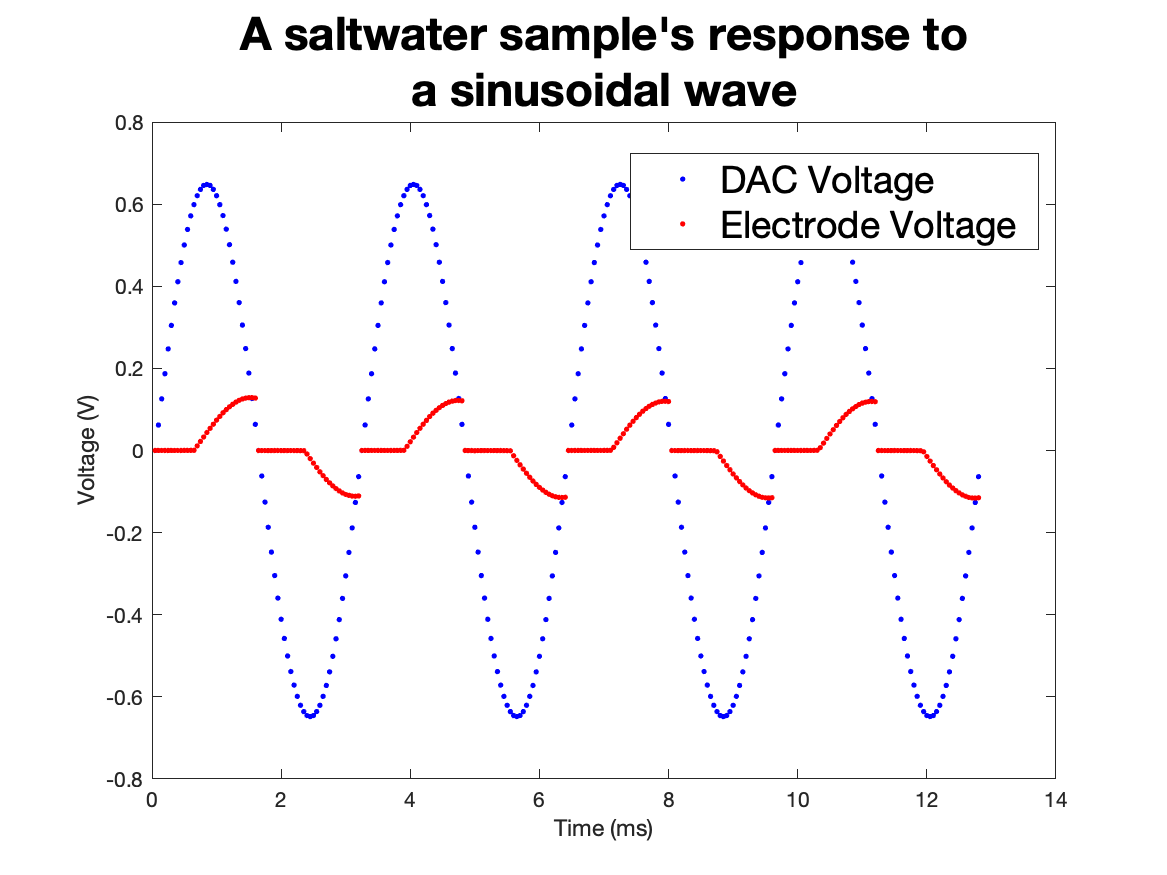
\includegraphics[width=\textwidth]{Figures/Testing/TiAC3}
        \caption{\gls{ac} test 1 with a 4 $250Hz$ sine waves centred at $0V$ on a $34,8$ \gls{psu} sample.}
        \label{fig:test19} %chktex 24
    \end{minipage}
    \begin{minipage}{0.5\textwidth}
        \centering
        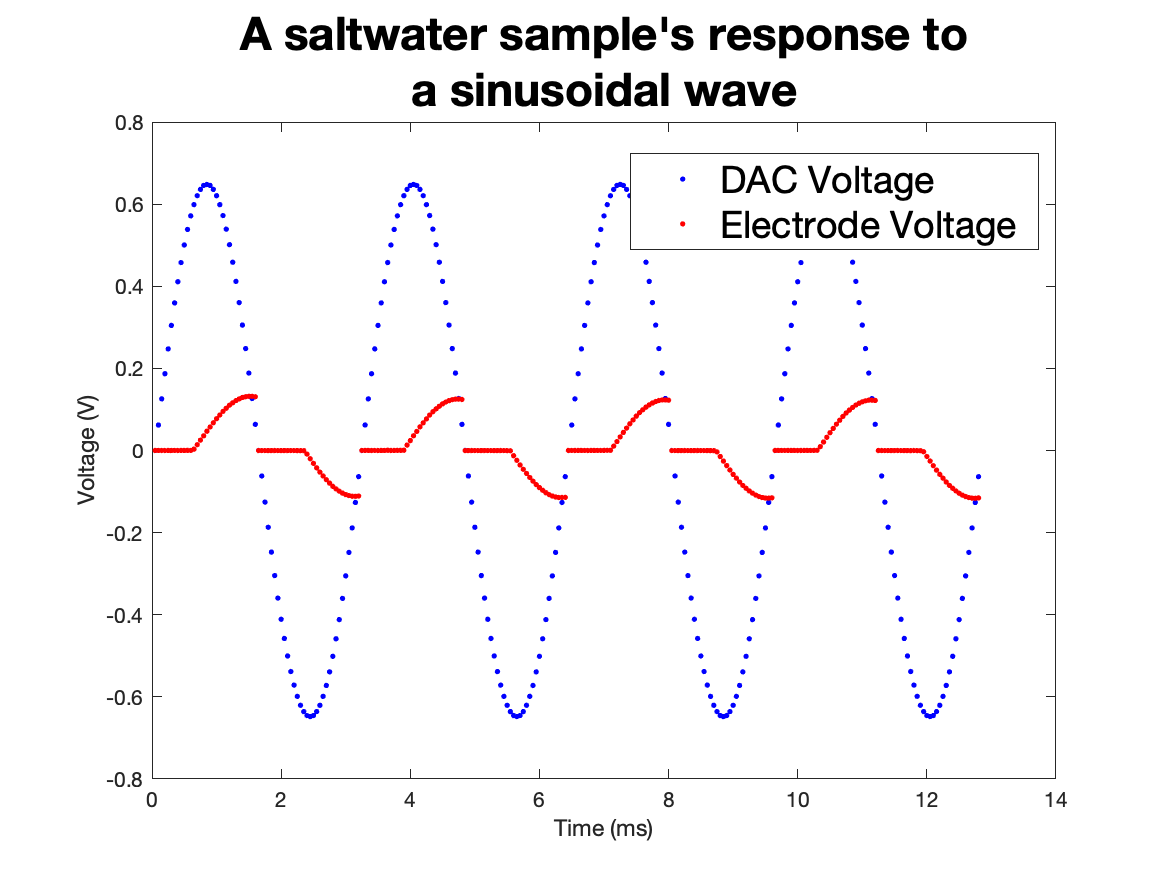
\includegraphics[width=\textwidth]{Figures/Testing/TiAC4}
        \caption{\gls{ac} test 1 with a 4 $250Hz$ sine waves centred at $0V$ on a $24,4$ \gls{psu} sample.}
        \label{fig:test20} %chktex 24
    \end{minipage}
\end{figure}

These tests showed no discernable difference between the amplitude and phase of the two samples.
This was likely due to the added capacitors affecting the response, and would need to be further investigated by first removing them before casting the probe into epoxy.
Unfortunately, the time limitations of the project prevented this from being attempted.